%\documentclass[ShortAfour,twocolumn,sageh]{sagej}
%\documentclass[journal]{IEEEtran}
\documentclass[twocolumn,authoryear,5p]{elsarticle}

%\usepackage[numbers,super]{natbib}
%\usepackage{cite} % for IEEEtran
%\usepackage{amsthm}
\usepackage{amsfonts}
\usepackage{amssymb}
\usepackage{mathtools}
\usepackage{graphicx}
\usepackage{color}
\usepackage{subcaption} 
\usepackage[bottom]{footmisc}
\usepackage{amsmath}
\usepackage[noabbrev]{cleveref}
%\usepackage{autonum} % looks weird maybe optimize?
\usepackage{mdframed}
\usepackage{booktabs}
\usepackage{picins}
%\usepackage{hyperref}
%\usepackage[caption=false,font=footnotesize]{subfig}
%\usepackage{stfloats} % invasive float package

\usepackage{pgfplots}
\pgfplotsset{compat=newest}
%% the following commands are needed for some matlab2tikz features
\usetikzlibrary{plotmarks}
%\usetikzlibrary{arrows.meta}
\usepgfplotslibrary{patchplots}
\usepackage{grffile}
%\mathtoolsset{showonlyrefs=true} % incompatible with cleveref
\usepackage{sectsty}
%\usepackage{titlesec}
%\allsectionsfont{\sffamily}
\usepackage[font={small,sf}]{caption}
\sectionfont{\large}
\subsectionfont{\normalfont\large\itshape}
\paragraphfont{\normalsize}

%\titleformat{\section}{\LARGE\bfseries}
%\titleformat{\subsection}{\Large\bfseries}
%\titleformat{\subsubsection}{\large\bfseries}
%\titleformat{\paragraph}{\large\bfseries}
%\titleformat{\subparagraph}{\large\bfseries}

%% you may also want the following commands
\pgfplotsset{plot coordinates/math parser=false}
\newlength\figureheight
\newlength\figurewidth

% theorem environment
\newtheorem{prop}{Proposition}[section]
\newtheorem{theorem}{Theorem}[section]
\newtheorem{prop2}{Proposition}
\newtheorem{lem}{Lemma}
\newtheorem{ex}{Example}

% For algorithms
\usepackage{algorithm}
\usepackage{algpseudocode}
\algnewcommand\algorithmicAnd{\textbf{and} }

\newlength\myindent
\setlength\myindent{2em}
\newcommand\bindent{%
  \begingroup
  \setlength{\itemindent}{\myindent}
  \addtolength{\algorithmicindent}{\myindent}
}
\newcommand\eindent{\endgroup}

% custom commands
\newcommand{\boldvec}[1]{\boldsymbol{\mathrm{#1}}}
\let\vec\boldvec
\newcommand\at[2]{\left.#1\right|_{#2}} % the at differential sign
\newcommand\scalemath[2]{\scalebox{#1}{\mbox{\ensuremath{\displaystyle #2}}}} % scaling matrices
\newcommand{\rpm}{\raisebox{.2ex}{$\scriptstyle\pm$}} % plus minus sign
\def\CC{{C\nolinebreak[4]\hspace{-.05em}\raisebox{.4ex}{\tiny\bf ++}}}

%% custom macros
\newcommand{\diag}{\mathop{\rm diag}}
\newcommand{\Alg}{\emph{Focused Player}}
\newcommand{\alg}{\mathrm{FP}} % first player
\newcommand{\AlgTwo}{\emph{Defensive Player}}
\newcommand{\algTwo}{\mathrm{DP}} % defensive player
\newcommand{\vhp}{\mathrm{VHP}} % virtual hitting plane based method

% % % % % % % % Notation for robot % % % % % % %
\newcommand{\todo}{\textcolor{red}{TODO}} % TODO!
\newcommand{\kin}{\vec{K}} % used to denote forward kinematics
\newcommand{\jac}{\vec{J}} % jacobian
\newcommand{\joint}{\vec{q}} % used to denote robot state in joint space
\newcommand{\invdyn}{\vec{f}} % used for inverse dynamics

% pos,vel and acc constraints
\newcommand{\jointMax}{\joint_{\mathrm{max}}}
\newcommand{\jointMin}{\joint_{\mathrm{min}}}
\newcommand{\velMax}{\dot{\joint}_{\mathrm{max}}}
\newcommand{\velMin}{\dot{\joint}_{\mathrm{min}}}
\newcommand{\accMax}{\ddot{\joint}_{\mathrm{max}}}
\newcommand{\accMin}{\ddot{\joint}_{\mathrm{min}}}

% % % % % % % % Table tennis notation % % % % % %
\newcommand{\resetTime}{0.5}
\newcommand{\numBallsMin}{N} % minimum number of balls to start prediction
\newcommand{\dataset}{\mathcal{D}}
\newcommand{\ball}{\vec{b}} % ball positions
%\newcommand{\ballEst}{\vec{b}_{\mathrm{est}}} % ball estimates (provided by EKF)
\newcommand{\ballPred}{\vec{b}} % ball prediction
\newcommand{\ballLand}{\vec{b}_{\mathrm{goal}}} % desired ball landing position
\newcommand{\ballVel}{v} 
\newcommand{\drag}{C_{D}} % drag coeff
\newcommand{\lift}{C_{L}} % lift coeff
\newcommand{\spin}{\vec{\omega}} % angular velocity
\newcommand{\gravityVec}{\vec{g}}
\newcommand{\coeffFrictionTable}{\mu_t} % dynamic coeff of friction
\newcommand{\coeffRestitutionTable}{\epsilon_t} % coeff of restitution between table and ball
\newcommand{\coeffRestitutionRacket}{\epsilon_r} % coeff of restitution between racket and ball
\newcommand{\gravity}{g}
\newcommand{\bounce}{\vec{A}_t} % bounce mat of table from ballvel to ballvel 
\newcommand{\bounceSpin}{\vec{B}_t} % bounce mat from ball spin to ballvel
\newcommand{\racketContact}{\vec{A}_r} % bounce mat of racket from ballvel to ballvel
\newcommand{\racketCartContact}{\bar{\vec{A}}_r} 
\newcommand{\racketContactSpin}{\vec{B}_r} % bounce mat of racket from spin to ballvel
\newcommand{\contactModel}{\vec{F}} % contact model
\newcommand{\racket}{\vec{r}} % racket positions
\newcommand{\racketVel}{\vec{v}} % racket velocity
\newcommand{\normal}{\vec{n}} % racket normal
\newcommand{\ballRadius}{r_{B}} % ball radius
\newcommand{\racketRadius}{r_{R}} % racket radius
\newcommand{\projRacket}{\vec{P}_{n}^{\perp}} % projection to axes perpendicular to normal
\newcommand{\minball}{12}
\newcommand{\ballPosEst}{\vec{b}_0} % estimated ball positions
\newcommand{\ballVelEst}{\vec{v}_0} % estimated ball velocities
\newcommand{\weightLand}{\alpha_{\mathrm{land}}} % weights for the landing penalty in Defensive Player
\newcommand{\weightHit}{\alpha_{\mathrm{hit}}} % weights for the hitting penalty in Defensive Player

% Environment limits and table tennis events
\newcommand{\tabletennis}{\mathcal{T}} % table
\newcommand{\landEvent}{\mathcal{L}} % landing event on opponents court
\newcommand{\net}{\mathcal{N}} % net
\newcommand{\hit}{\mathcal{H}} % hitting event
\newcommand{\xtablelim}{x_{\mathrm{max}}} % x limit of table
\newcommand{\ytablelim}{y_{\mathrm{max}}} % y limit of table assuming origin is center of table
\newcommand{\ztable}{z_{T}} % height of table
\newcommand{\znet}{z_{\mathrm{net}}} % height of net
\newcommand{\zwall}{z_{\mathrm{wall}}} % height of wall

% notation for times 
\newcommand{\hitTime}{T} % hitting or striking time
\newcommand{\restTime}{T_{\mathrm{rest}}} % returning time
\newcommand{\netTime}{T_{\mathrm{net}}} % time when ball flies over the net
\newcommand{\landTime}{T_{\mathrm{land}}} % landing time on table
\newcommand{\predTime}{T_{\mathrm{pred}}} % maximum prediction time for the ball

\newcommand{\hitFun}{\vec{\Psi}_{\mathrm{hit}}} % hitting function
\newcommand{\landFun}{\vec{\Psi}_{\mathrm{land}}} % landing function
\newcommand{\netFun}{\vec{\Psi}_{\mathrm{net}}} % net function

% Maximum principle notation
\newcommand{\sysInput}{\vec{u}} % control inputs
\newcommand{\hamiltonian}{\mathcal{H}} % hamiltonian
\newcommand{\momentaPos}{\vec{\lambda}} %generalized momenta for joint positions
\newcommand{\momentaVel}{\vec{\mu}} %generalized momenta for joint velocities


% Set the paths where all figures are taken from:
\graphicspath{{Figures/}}
%\mathtoolsset{showonlyrefs} 
\newcommand{\includesvg}[1]{%
% \executeiffilenewer{#1.svg}{#1.pdf}%
% {inkscape -z -D --file=#1.svg %
% --export-pdf=#1.pdf --export-latex}%
 \input{#1.pdf_tex}%
}

\setcounter{secnumdepth}{2}
%\setcounter{tocdepth}{3}

\begin{document}


\title{Online optimal trajectory generation for robot table tennis}
\author[tue]{Okan Ko\c c\corref{cor1}}
\ead{okan.koc@tuebingen.mpg.de}
\author[darm]{Guilherme Maeda}
\ead{maeda@ias.tu-darmstadt.de}
\author[tue,darm]{Jan Peters}% <-this % stops a space 
\ead{jan.peters@tuebingen.mpg.de}
\cortext[cor1]{Corresponding author}
\address[tue]{Max Planck Institute for Intelligent Systems, Spemannstr. 38, 72076 Tuebingen, Germany}
\address[darm]{Technische Universit\" at Darmstadt, FG Intelligente Autonome Systeme Hochschulstr. 10, 64289 Darmstadt, Germany}

%%%%% IEEE FORMAT
%\author{Okan Ko\c c$^{1}$, Guilherme Maeda$^{2}$ and Jan Peters$^{1,2}$% <-this % stops a space 
%\\
%{\tt\small \{okan.koc, jan.peters\}@tuebingen.mpg.de}%
%\thanks{$^{1}$Max Planck Institute for Intelligent Systems, Spemannstr. 38, 72076 Tuebingen, Germany}
%\thanks{$^{2}$Technische Universitaet Darmstadt, FG Intelligente Autonome Systeme Hochschulstr. 10, 64289 Darmstadt, Germany}
%}
%%%%% SAGE FORMAT
%\runninghead{Ko\c c, Maeda et al.}
%\author{Okan Ko\c c\affilnum{1}, Guilherme Maeda\affilnum{2} and Jan Peters\affilnum{1,2}}
%\affiliation{\affilnum{1}Max Planck Institute for Intelligent Systems\\ \affilnum{2}Technische Universitaet Darmstadt, FG Intelligente Autonome Systeme}
%\corrauth{Max Planck Institute for Intelligent Systems,
%        Spemannstr. 38, 72076 Tuebingen, Germany}
%\email{okan.koc@tuebingen.mpg.de}
%\maketitle

%%%%%%%%%%%%%%%%%%%%%%%%%%%%%%%%%%%%%%%%%%%%%%%%%%%%%%%%%%%%%%%%%%%%%%%%%%%
\begin{abstract}
%
% COMMENTS/CHANGES HERE
% To simplify the problem,  conventional planning algorithms
%
In highly dynamic tasks that involve moving targets, planning is necessary to figure out when, where and how to intercept the target. In robotic table tennis in particular, motion planning can be very challenging due to time constraints, dimension of the search space and joint limits. Conventional planning algorithms often rely on a fixed virtual hitting plane to construct robot striking trajectories. These algorithms, however, generate restrictive strokes and can result in unnatural strategies when compared with human playing. In this paper, we introduce a new trajectory generation framework for robotic table tennis that does not involve a fixed hitting plane. A free-time optimal control approach is used to derive two different trajectory optimizers. The resulting two algorithms, Focused Player and Defensive Player, encode two different play-styles. We evaluate their performance in simulation and in our robot table tennis platform with a high speed cable-driven seven DOF robot arm. The algorithms return the balls with a higher probability to the opponent's court when compared with a virtual hitting plane based method. Moreover, both can be run online and the trajectories can be corrected with new ball observations.
%To improve performance, parameters of the ball prediction models are estimated from human demonstrations. The resulting trajectories have lower accelerations while the joint constraints are enforced at all times. 

\end{abstract}

%%%%%%%%%%%%%%%%%%%%%%%%%%%%%%%%%%%%%%%%%%%%%%%%%%%%%%%%%%%%%%%%%%%%%%%%%%%

%\begin{IEEEkeywords}
%Optimal Control, Motion Planning, Optimization, Robot Table Tennis
%\end{IEEEkeywords}
%\keywords{Optimal Control, Motion Planning, Optimization, Robot Table Tennis}
\begin{keyword}
Optimal Control \sep Motion Planning \sep Optimization \sep Robot Table Tennis
\end{keyword}
\maketitle

\section{Introduction}

% It is a challenging testbed for robotics algorithms
Table tennis is a challenging game for humans to master. For robots, it also serves as a testbed to study and validate the effectiveness of different movement generation algorithms. Combining different estimation, movement generation and execution schemes and studying how close they come to imitating expert human behaviour will yield important insights for robotics research.

Optimality plays an important role in the search for efficient and feasible striking trajectories. However, so far most of the research in robotic table tennis were based on specialized systems, such as Cartesian coordinate robots \citep{Matsushima05,Yanlong13}, that eliminate great part of the difficulties in trajectory generation. Furthermore, most algorithms for robotic table tennis focused on simplifications of the game that reduced the dimensions of the search space \citep{Muelling11} in order to quickly come up with a movement plan. In this paper, we show the advantages of incorporating optimality in trajectory generation to create more flexible movement. 
% refs needed

% GOOD SOUNDS A BIT INFORMAL
Our robotic setup with an anthropomorphic seven degree of freedom Barrett WAM arm is shown in Figure~\ref{robot}. The redundant arm can achieve high speeds and accelerations. It is a good platform to study different movement generation schemes. Optimal control based approaches have the potential to make use of all degrees of freedom in planning, contributing to more natural and efficient generation of strikes. % ref needed
%
The contributions of this paper are as follows: first, we introduce an optimal control framework in robot table tennis where the generation of striking trajectories is the result of an optimization problem. As opposed to previous works, inverse kinematics or a fixed plane to compute joint trajectories are not needed. Two different optimization approaches are presented that encode defensive and goal-oriented styles of playing. We show extensive experiments in simulation and on our table tennis platform, where we evaluate and compare the performance of the algorithms. We do not rely on pure physical modeling to compute desired ball and racket parameters. Instead, the parameters of the prediction models are estimated based on human ball-racket demonstrations.
%
\begin{figure}[t]
	\center
	\includegraphics[scale=0.4]{robot1.png}			
	\caption{Robotic table tennis setup with four cameras on the corners of the ceiling tracking the ball at 60 Hz. We present two optimal control based trajectory generation algorithms that encode defensive and goal-oriented styles of playing. A constrained nonlinear optimization problem is solved in both cases to find an optimal striking trajectory as well as an optimal striking time.	
		%The raw ball data provided from the cameras is filtered with an Extended Kalman Filter and the future path of the ball is predicted.
	}
	\label{robot}
\end{figure}
\subsection{Related Work}\label{relatedWork}

One of the most popular frameworks in table tennis is the Virtual Hitting Plane (VHP) method, which is based on the virtual hitting point hypothesis~\citep{Ramanantsoa94}. In this approach, the trajectory of an incoming ball is first estimated from a stream of ball position observations. Usually, a physical flight model is then used to predict the intersection point of the future ball trajectory with an appropriately chosen plane along the vertical axis. This procedure determines the striking time as well as the striking point. The remaining task-space parameters, the desired racket velocity and normal at striking time, are determined by running the physical flight model backwards from a desired ball landing position and velocity, and inverting the ball-racket contact model. For a more general discussion, see \citet{Matsushima05} and \citet{Muelling11}. A clear limitation of the method is shown in Figure~\ref{mainIdea}. A player fixing the VHP may not generate feasible trajectories for some ball trajectories. By means of trajectory optimization, trajectories can be generated that are not constrained to a hitting plane.

% THE EMBODIMENT PROBLEM
Another framework that uses a mixture of movement primitives and reinforcement learning is given in~\citet{Muelling13}. Initialized with a set of dynamic movement primitives (DMP) extracted from demonstrations, reinforcement learning is applied to select and generalize between the teach-in movements. A problem with this approach is that not all robots can be trained well this way. For example, the shoulder of the robot shown in Figure~\ref{robot} weighs $10$ kg alone, and the wrist weighs about $2.5$ kg. It is more difficult to move the links with heavy inertia, whereas it is easier to find optimization algorithms that make use of them.

%For safety reasons, a minimum hitting time $T_{\mathrm{min}}$ is also specified in addition to the coordinates of the hitting plane. The estimation process has to be terminated at least $T_{\mathrm{min}}$ seconds before the expected hitting time, to give the robot enough reaction time. This prevents high accelerations and any risk of damage to the robot. 

A related dynamic framework involving moving targets is the ball catching robot of~\citet{Baeuml11} where a computationally demanding optimization problem is solved online. It includes also the catching time as another parameter to be optimized. The framework of~\citet{Kim10} considers generating catching movements for more general objects. Another application of optimal control showing the benefits of spatio-temporal optimization is given in~\citet{Nakanishi2016} on a brachiating robot. The computed solutions require lower torques when compared with traditional optimal control approaches fixing the time interval. 
% more refs especially the polynomial generation framework cited in Billard's paper
%Robustness of a paddling task is analyzed in~\cite{Burridge99}. 

In the remainder of this paper, the framework is described in detail. Robot trajectory generation for table tennis is formalized as an optimal control problem in Section~\ref{ps}. Two efficient solvers are presented in Sections~\ref{method} and~\ref{method2} for optimizing the cost functional under additional constraints. The performance of the two resulting players are evaluated in Section~\ref{results} and it is shown that they compare favorably with an inverse kinematics based approach in simulation. Physical ball models are used to predict the future ball trajectory, and in Section~\ref{sectionPredict} estimation of the parameters of these models from actual data is discussed. Finally, real robot experiments are shown, where the algorithms run online in the table tennis setup. Based on this evaluation, conclusions are given with several promising extensions which might be necessary to increase performance further. Parts of this paper appeared in \citet{Koc16}, where one of the algorithms ($\Alg$) was proposed and evaluated in simulation. A lookup table based approach was suggested to implement it online in the table tennis platform.

\begin{figure}[t!]
\centering
\includegraphics[scale=0.30]{drawingUpdate.eps}			
\caption{Fixing a virtual hitting plane (VHP) can make the generated trajectories unnecessarily restrictive and the resulting inverse kinematics may be infeasible. Instead the whole ball trajectory should be considered in a trajectory generation framework and the hitting time as well as the hitting point should be optimized. The predicted ball trajectory and a feasible racket trajectory are shown in red and black, respectively. VHP is shown as a dotted gray line, the workspace of the robot is shown as an ellipsoidal light blue region.}
\label{mainIdea}
\end{figure}
\subsection{Problem Statement}\label{ps}

Most of the algorithms for robotic table tennis need to specify when, where and how to intercept the incoming ball trajectory $\ball(t)$. In \citet{Matsushima05} and \citet{Muelling11} for example, the authors calculate the intersection point of a predicted ball trajectory $\ballPred(t)$ with a virtual hitting plane (VHP) at $y = y_{\mathrm{VHP}}$ to determine the space and time coordinates of the hitting event. Although additional constraints like the VHP can simplify trajectory generation, they can also lead to awkward or infeasible movements. It is possible to eliminate this plane altogether and include the striking time as another parameter to be determined in an optimization problem.

%
%\subsection{Optimal Control for Trajectory Generation}
%
When generating striking trajectories for a robot with $n$ degrees of freedom, trajectories with minimal acceleration can be preferred for safety and efficiency reasons. Consider the following \emph{free-time} optimal control problem~\citep{Liberzon11}
%
\begin{align}
\min_{\ddot{\joint},T} & \int\limits_{0}^{T} \ddot{\joint}(t)^{\mathrm{T}}\vec{R}\ddot{\joint}(t) \ \mathrm{d}t \label{costFnc1} \\
\text{s.t. }  
&\hitFun\big(\joint(\hitTime),\hitTime\big) \in \hit, \label{hitFunc} \\
&\netFun\big(\joint(\hitTime),\dot{\joint}(\hitTime),\hitTime\big) \in \net, \label{netFunc} \\
&\landFun\big(\joint(\hitTime),\dot{\joint}(\hitTime),\hitTime\big) \in \landEvent, \label{landFunc} \\
& \joint(0) = \joint_{0}, \label{initCond1} \\
& \dot{\joint}(0) = \dot{\joint}_{0}, \label{initCond2}
\end{align}
%
\noindent where the final hitting time $\hitTime$ is an additional variable to be optimized along with the joint accelerations $\ddot{\joint}(t) \colon [0,\hitTime] \to \mathbb{R}^{n}$. The weighting matrix $\vec{R}$ for the accelerations is positive definite. %i.e., $\vec{R} \succ 0 \in \mathbb{R}^{n \times n}$. 
Initial conditions for the robot are the joint positions $\joint_0$ and joint velocities $\dot{\joint}_0$.
%$\vec{T}(\cdot) \in \mathbb{R}^{4 \times 4}$ 
The inequality constraints \mbox{\eqref{hitFunc} -- \eqref{landFunc}} ensure that the task requirements for table tennis are satisfied. The hitting constraint $\hitFun \in \hit$ ensures impact of the racket with the ball at striking time $T$. The net constraint $\netFun \in \net$ makes sure the ball passes over the net and finally, the landing constraint $\landFun \in \landEvent$ captures the requirement that the ball should bounce first on the opponents court. See Figure~\ref{tableTennisConstraints} for an illustration. The precise definitions of these constraint functions and the constraint sets will be introduced in section~\ref{method2}.
% These algorithms can possibly lead to different play styles, depending on the higher level strategy.

Solutions of \mbox{\eqref{costFnc1} -- \eqref{initCond2}} can be found using Pontryagin's minimum principle~\citep{Pontryagin}. The optimal $\joint(t)$ in both cases is a third degree polynomial for each degree of freedom, with the inequality constraints \mbox{\eqref{hitFunc} -- \eqref{landFunc}} imposing generalized \emph{transversality conditions} on the Hamiltonian and the momenta to satisfy at striking time~\citep{BrysonHo69,Schaettler12}. Solving such boundary value problems is hard, especially given real time constraints. In the later sections we will introduce two algorithms that will solve this problem efficiently under additional constraints. These two approaches can be seen as different ways to solve the underlying table tennis task efficiently and they lead to two different play-styles. 

%See Figure~\ref{mainIdea} for an illustration.

When given only constraints at the boundary, the striking time $T$, the joint position and velocity values at striking time $\joint_f$ and $\dot{\joint}_f$ fully parametrize this problem. The polynomial coefficients for the striking trajectory
%
\begin{align}
\joint_{\mathrm{strike}}(t) = \vec{a}_3 t^3  + \vec{a}_2 t^2 + \dot{\joint}_0 t + \joint_0, 
\end{align} %\ 0 \leq t \leq T,
%
\noindent can then be determined in joint-space for each degree of freedom of the robot
%can be parameterized in terms of final joint positions $\joint_f$, final joint velocities $\dot{\joint}_f$ and striking time $T$
%
\begin{gather}
\begin{aligned}
\vec{a}_3 &= \frac{2}{T^3}(\joint_0 - \joint_f) + \frac{1}{T^2}(\dot{\joint}_0 + \dot{\joint}_f), \\
\vec{a}_2 &= \frac{3}{T^2}(\joint_f - \joint_0) - \frac{1}{T}(\dot{\joint}_f + 2\dot{\joint}_0).
\label{coeffs}
\end{aligned}
\end{gather}
%
% After computing the parameters $T, \joint_f, \dot{\joint}_f$, we generate also a returning trajectory $\joint_{\mathrm{return}}(t)$ to the same initial posture $\joint_0$ with an appropriately chosen return time $\returnTime$. The return time can be chosen sufficiently long to guarantee feasibility of the returning trajectory. 

The notation that is used frequently in the rest of the paper is shown in Table~\ref{tableSymbols} for the reader's convenience.
%Initially the robot will not be moving, $\dot{\joint}_0 = 0$.
%
\begin{figure}
	\centering
	\includegraphics[width=0.5\textwidth]{tableTennisConstraints.pdf}%
	\caption{In table tennis, robot trajectories (blue) can be seen as reactions to predicted ball trajectories (orange). The players are free to decide where, when and how to intercept the ball. However, the resulting outgoing ball trajectories need to be \emph{feasible}: the ball has to pass above the net and land on the opponent's court. The feasible region above the net is drawn in transparent green. The rules of the game can be captured as constraints for generating robot striking trajectories.}
	\label{tableTennisConstraints}
\end{figure}
%
%
\begin{figure*}
	\centering
	\def\svgwidth{2.0\columnwidth}
	\input{Figures/predictionModels.pdf_tex}
	%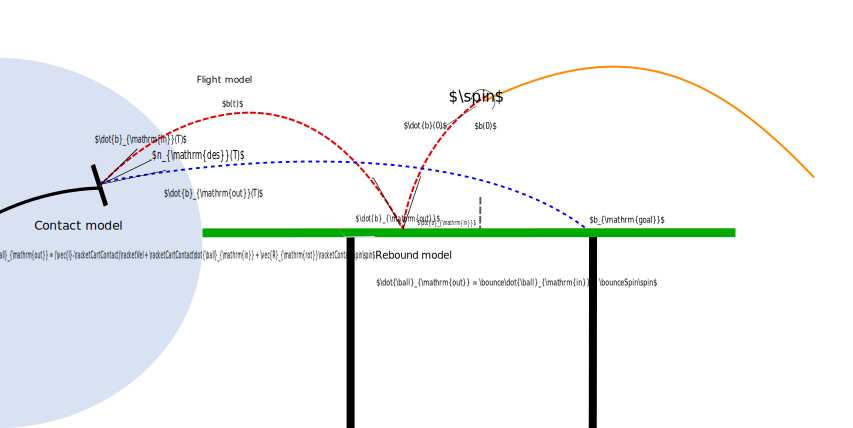
\includegraphics[width=0.8\textwidth]{predictionModels.pdf}%
	\caption{Ball prediction schema for table tennis. After estimating the initial ball position, velocity and spin, the future path of the ball can be predicted using the flight model, the rebound model and the racket-ball contact model. The trajectory generation framework uses these models to compute desired striking trajectories.}
	\label{tableTennisSchema}
\end{figure*}
%
%
\begin{table}[b!]
	\small\sf\centering
	%\renewcommand{\arraystretch}{1.3}
	\caption{Table of Symbols}
	\label{tableSymbols}
	\resizebox{\columnwidth}{!}{%
	\begin{tabular}{c|l}
		%\hline
		\toprule
		\bfseries Notation & \bfseries Explanation \\ %	{\small \bfseries Notation}
		\midrule
		%\hline
		$\hitTime$ & hitting time \\
		$\restTime$ & return time \\
		$\landTime$ & desired ball landing time after hit \\
		%$\predTime$ & prediction horizon for incoming ball \\
		$\ballLand$ & desired ball landing positions \\
		$\joint(t)$ & joint trajectory \\
		$\ballPred(t)$ & predicted ball trajectory \\
		$\racket(t)$ & racket center position \\
		$\racketVel(t)$ & racket velocity \\
		$\normal(t)$ & racket normal \\
		$\kin_p$ & kinematics function for racket center position \\ 
		$\kin_n$ & kinematics function for racket normal \\
		$\jac(\joint_f)$ & jacobian at hitting time \\                 
		$\normal_{\mathrm{des}}(T)$ & desired racket normal at hitting time \\
		$\racketVel_{\mathrm{des}}(T)$ & desired racket velocity at hitting time \\
		$\spin$ & ball spin \\
		$\dot{\ball}_{\mathrm{in}}, \dot{\ball}_{\mathrm{out}}$ & ball velocity before and after impact \\
		$\numBallsMin$ & minimum number of balls to start prediction \\
		$\joint_0, \dot{\joint}_0$ & initial joint positions and velocities \\
		$\joint_{\mathrm{cur}}, \dot{\joint}_{\mathrm{cur}}$ & joint position and velocity estimates \\
		$\joint_f, \dot{\joint}_f$ & joint position and velocity at hitting time \\
		$\joint_{\mathrm{ext}}$ & joint extreme values of trajectory \\
		$\jointMax, \jointMin$ & joint angle upper and lower limits \\
		$\vec{R}$ & weighting matrix \\
		$\joint_{\mathrm{strike}}(t)$ & joint striking trajectory \\
		$\joint_{\mathrm{return}}(t)$ & joint returning trajectory \\
		$\hitFun,\landFun, \netFun$ & table tennis task constraints \\
		%$\joint_{\mathrm{des}}$ & strike \& return trajectory \\
		%$\vec{\tau}$ & torques computed by inverse dynamics \\
		%\bottomrule
	\end{tabular}
}
\end{table}
%
\subsection{Background on Ball Prediction}\label{sectionPredict} % Predicting with Ball Models
 
For the trajectory generation process, three ball models will be used to determine the table tennis task constraints \mbox{\eqref{hitFunc} -- \eqref{landFunc}}: ball flight model, ball-table rebound model and ball-racket contact model. Whenever an incoming ball is detected in midair, a flight model will first be used to predict the trajectory $\ballPred(t)$ of the ball centre of mass coordinates $\ball = (b_x,b_y,b_z)^{\mathrm{T}}$ until impact with a racket, table or ground. 

\paragraph{Flight model.} Table tennis balls are very light, a standard ball weighs about $2.7$ grams, which makes nonlinear effects due to air drag and spin noticeable especially when the ball speed $\ballVel = \|\dot{\ball}\|_2$ is high. The \emph{flight model}~\citep{Nakashima10}
%
\begin{align}
%\big(\ddot{b}_x, \ddot{b}_y, \ddot{b}_z\big)^{\intercal} = \big(-\drag \ballVel \dot{b}_x, -\drag \ballVel \dot{b}_y, \gravity - \drag \ballVel \dot{b}_z\big)^{\intercal} \label{flightModel}
\ddot{\ballPred} = \gravityVec -\drag\ballVel \, \dot{\ballPred} + \lift \spin \times \dot{\ballPred}, \label{flightModel}
\end{align}
%
\noindent is a nonlinear dynamics model that incorporates air drag and spin effects. The air drag constant $\drag$ and the lift constant $\lift$ as well as gravity $\gravity$, $\gravityVec = (0,0,\gravity)^{\mathrm{T}}$, parameterize this model. The \emph{magnus effect} due to spin (angular velocity) $\spin$, for example, acts as an additional downward force for an incoming ball if the angular velocities are in the negative $x$-direction (topspin). It is assumed that spin stays constant throughout the ball motion.
%
\paragraph{Rebound Model.} Formally, rebound is a discrete event which reflects the ball velocity when the ball hits the table. The incoming velocities  $\dot{\ball}_{\mathrm{in}}$ at bouncing time are transformed to outgoing velocities $\dot{\ball}_{\mathrm{out}}$. The following nonlinear \emph{rebound model}~\citep{Nakashima10} for a standard ball with radius $\ballRadius = 2$ cm,
%
\begin{align}
\dot{\ball}_{\mathrm{out}} = \bounce\dot{\ball}_{\mathrm{in}} + \bounceSpin\spin,
\label{reboundModel}
\end{align}
%
\noindent is parameterized by the dynamic coefficient of friction $\coeffFrictionTable$ and the coefficient of restitution $\coeffRestitutionTable$ of the table
%
\begin{align}
\scalemath{0.9}{\bounce} &= \scalemath{0.8}{\begin{bmatrix}
1 - \alpha & 0 & 0 \\
0 & 1 - \alpha & 0 \\
0 & 0 & -\coeffRestitutionTable
\end{bmatrix}} , \
\scalemath{0.9}{\bounceSpin} = \scalemath{0.8}{\begin{bmatrix}
0 & \alpha\ballRadius & 0 \\
-\alpha\ballRadius & 0 & 0 \\
0 & 0 & 0
\end{bmatrix}},
\end{align}
%
\noindent where the nonlinearity comes from the term
%
\begin{align}
\alpha &= \coeffFrictionTable(1 + \coeffRestitutionTable)\tfrac{\dot{b_z}}{\|\dot{\ball}_T\|},
\end{align}
%
\noindent $\dot{\ball}_T$ is the \emph{tangent velocity} at contact
%
\begin{align}
\dot{\ball}_T &= (\dot{b}_x - \ballRadius \omega_y, \dot{b}_y + \ballRadius \omega_x, 0)^{\mathrm{T}},
\end{align}
%
\noindent for $\spin = (\omega_x, \omega_y, \omega_z)^{\mathrm{T}}$. This model suggests, for example, that some amount of topspin is transferred at sliding impact to linear velocity in the y-direction. See Figure~\ref{tableTennisSchema} for a table tennis schema. 

\paragraph{Racket Contact Model.}  We assume the following linear racket contact model holds for a standard racket with radius $\racketRadius \approx 7.6$ cm,
%
\begin{align}
\vec{o} = \racketContact\vec{i} + \racketContactSpin\spin,
\label{contactModel}
\end{align}
%
\noindent between the outgoing ball velocity $\vec{o}$ and the incoming ball velocity $\vec{i}$, similar to~\eqref{reboundModel} but in the moving racket frame. The outgoing ball Cartesian velocities are hence found by multiplying $\vec{o}$ with the racket rotation matrix and adding the racket velocities, i.e., $\dot{\ball}_{\mathrm{out}}(t) = \vec{R}_{\mathrm{rot}}\vec{o}(t) + \racketVel(t)$, where the rotation matrix $\vec{R}_{\mathrm{rot}}(\joint(t))$ of the racket is given by the kinematics function. The impact model is parameterized by the constants $\kappa$ and $\coeffRestitutionRacket$
%
\begin{align}
\scalemath{0.8}{\racketContact} &= \scalemath{0.8}{\begin{bmatrix}
1 - \kappa & 0 & 0 \\
0 & 1 - \kappa & 0 \\
0 & 0 & -\coeffRestitutionRacket
\end{bmatrix}}, \ 
\scalemath{0.8}{\racketContactSpin} = \scalemath{0.8}{\begin{bmatrix}
0 & \kappa\racketRadius & 0 \\
-\kappa\racketRadius & 0 & 0 \\
0 & 0 & 0
\end{bmatrix}}.
\label{racketMatrices}
\end{align}
%
Letting $\racketCartContact := \vec{R}_{\mathrm{rot}}\racketContact\vec{R}_{\mathrm{rot}}^{\mathrm{T}}$, we get the following relationship between the Cartesian velocities:
%
\begin{align}
\dot{\ball}_{\mathrm{out}} = (\vec{I}-\racketCartContact)\racketVel + \racketCartContact\dot{\ball}_{\mathrm{in}} + \vec{R}_{\mathrm{rot}}\racketContactSpin\spin.
\end{align}

%
%racket velocity $\racketVel$ and racket normal $\normal$. Equation~\eqref{contactModel} is a generalization of the \emph{mirror law}~\cite{Muelling11}, where the outgoing velocity of the ball as a result of contact is calculated as a simple reflection %The matrix $\contactModel \in \mathbb{R}^{3 \times 9}$
%%
%\begin{align}
%o_{n} - v_{n} = -\epsilon_{R} (i_{n} - v_{n}),
%\label{mirrorLaw}
%\end{align}
%%
%\noindent with $v_{n}$ the speed of the racket along its normal $\normal(t)$ and $\epsilon_{R} \in [0,1]$ the coefficient of restitution of the racket. Scalars $o_{n}$ and $i_{n}$ are the outgoing and incoming ball speeds along the racket normal, respectively. This model \eqref{mirrorLaw} assumes an elastic momentum exchange and in our experience, it is quite inaccurate, especially at high ball velocities, as will be shown empirically in section~\ref{results}.

\paragraph{Ball Prediction.} The models~\mbox{\eqref{flightModel} -- \eqref{racketMatrices}} can be composed together to predict the future ball trajectory given camera observations. We use an Extended Kalman Filter (EKF) to estimate the ball state from observations~\citep{Sorenson85}. The ball state for the filter is the ball positions and velocities, since we assume that the ball spin is constant throughout motion. The ball spin can be seen as a parameter of the prediction functions. 
% Any other regression method to estimate initial ball position and velocity can also be used. 

EKF instantiated with the models~\eqref{flightModel} -- \eqref{racketMatrices}, the initial ball positions $\ball_0$ and velocities $\dot{\ball}_0$ and spin $\spin$, estimates the evolving ball state and predicts the future ball trajectory at each time instant $t$: a multivariate normal distribution $p_t(\ball,\dot{\ball})$ of ball states parameterized by time is generated
%
\begin{align}
\big(\ball(t)^{\intercal},\dot{\ball}(t)^{\intercal}\big)^{\intercal} &\sim p_t(\ball,\dot{\ball}) = \mathcal{N}(\vec{\mu}(t),\vec{\Sigma}(t)),
%\label{ballProcess}
\end{align}
%
\noindent where $\vec{\mu}(t) = \big(\ballPred(t)^{\intercal},\dot{\vec{b}}(t)^{\intercal}\big)^{\intercal}$ is the mean ball position and velocity predictions. The covariance matrix $\vec{\Sigma}(t)$ is updated along with the mean estimate $\vec{\mu}(t)$ using the EKF predict and update equations. The covariance matrices are used to reject outliers and hence make Kalman Filtering more robust to ball detection errors.
%This typically happens when the vision system~\citep{Lampert12} cannot reliably detect a flying orange ball in the image.
% among other things

\section{The Focused Player}\label{method}

A higher-level strategy in table tennis could, based on a perceived state of the opponent, command to return an incoming ball to a desired location. A reliable trajectory generation algorithm for that purpose should be flexible and easily find safe joint movements. The optimal control based approach penalizing sum of squared accelerations, in this regard, leads to a flexible optimization problem where it is easy to find good hitting postures, while satisfying additional safety constraints. 

\subsection{Racket Constraints}
%
The optimal control problem introduced in~\eqref{costFnc1} can be solved efficiently under additional racket constraints
%
%Fixing a desired landing position $\ballLand$ and time $\landTime$ converts the table tennis task constraints into Cartesian equality constraints. By running the ball flight model backwards and inverting the ball-racket contact model we get the following equalities
%
\begin{align}
& \kin_p(\joint(T)) = \ballPred(T), \label{transCond1} \\
& \kin_n(\joint(T)) = \normal_{\mathrm{des}}(T), \label{transCond2}\\
& \jac(\joint(T))\dot{\joint}(T) = \racketVel_{\mathrm{des}}(T), \label{transCond3}
\end{align}
%
that guarantee the return of the incoming ball to a desired location at a desired landing time. The racket center position $\racket(\hitTime)$ and the racket normal $\normal(\hitTime)$ at hitting time $\hitTime$ are computed using the kinematics functions $\kin_p(\cdot)$ and $\kin_n(\cdot)$, respectively. The Jacobian $\jac(\cdot) \in \mathbb{R}^{3 \times n}$ \citep{Spong06} at hitting time transforms the joint velocities in \eqref{transCond3} into racket velocities $\racketVel(T)$. 

The Cartesian task constraints~\mbox{\eqref{transCond1} -- \eqref{transCond3}} can satisfy and hence effectively replace the table tennis task constraints \mbox{\eqref{hitFunc} -- \eqref{landFunc}} for suitable $\normal_{\mathrm{des}}(T), \racketVel_{\mathrm{des}}(T)$. To maximize the probability of hitting the ball, the desired racket center is set at hitting time equal to the mean ball position estimate in \eqref{transCond1}, i.e., $\racket(T) = \ballPred(T)$. To return the ball to the opponent's court, the constraints on the racket normal $\normal(\hitTime)$ and velocity at hitting time $\racketVel(\hitTime)$ are imposed. 
%
%
\paragraph{\textbf{Calculating Desired Racket Parameters}.}\label{calcDesRacket} After predicting the future ball path $\ballPred(t)$, the next step is to compute desired racket velocities $\racketVel_{\mathrm{des}}(t)$ and desired racket normals on this path $\normal_{\mathrm{des}}(t)$. These desired racket parameters will give the incoming ball during the impact, a desired outgoing ball velocity according to~\eqref{contactModel}. They are calculated by first specifying a desired landing point $\ballLand$ and a desired time duration $\landTime$. A desired ball outgoing velocity is then found by solving the boundary value problem for the flight model~\eqref{flightModel} with the boundary values
%
\begin{gather}
\begin{aligned}
&\ball_{\mathrm{out}}(0) = \ballPred(t), \\
&\ball_{\mathrm{out}}(\landTime) = \ballLand,
\label{bvp}
\end{aligned}
\end{gather}
%
\noindent for each $t$. Afterwards, $\racketVel_{\mathrm{des}}(t)$ and $\normal_{\mathrm{des}}(t)$ are calculated by inverting the racket contact model~\eqref{contactModel} given the outgoing ball velocities $\dot{\ball}_{\mathrm{out}}$ at impact.
% TODO: talk about the inversion in more detail.

In practice, \eqref{bvp} can be solved very fast for each $t$ by initializing it with the closed form solution of the ballistic flight model (i.e., zero drag and spin). 
%
%The vector-valued functions $\kin_p(\cdot), \kin_n(\cdot) \in \mathbb{R}^{3 \times 1}$ are the relevant submatrices of the direct kinematics function~\citep{Spong06} giving the racket center position $\racket(T)$ and the racket normal $\normal(T)$ at striking time $T$ respectively.
%
\subsection{Nonlinear Constrained Optimization}\label{nco1}
%
We briefly show here that the solution $\joint(t)$ to the optimal control problem posed in \eqref{costFnc1} under additional racket constraints~\mbox{\eqref{transCond1} -- \eqref{transCond3}} is a third order polynomial for each degree of freedom, $i = 1, \ldots, n$. 
%
\paragraph{\textbf{Derivation from Maximum Principle}.} Using the maximum principle for unconstrained inputs $\sysInput(t) = \ddot{\joint}(t) \in \mathbb{R}^{n}$, the Hamiltonian 
%
\begin{align}
\hamiltonian(\sysInput,\dot{\joint},t) = \sysInput^{\mathrm{T}}\vec{R}\sysInput(t) + \momentaPos^{\mathrm{T}}\dot{\joint} + \momentaVel^{\mathrm{T}}\sysInput
\end{align}
%
\noindent for the momenta $[\momentaPos(t),\momentaVel(t)] \in \mathbb{R}^{2n}$ is minimized at 
%
\begin{align}
\sysInput^{*}(t) = -\frac{1}{2} \vec{R}^{-1}\momentaVel^{*}(t).
\label{HamiltonianMaxInput}
\end{align}
%
Costate equation for the momenta gives
%
\begin{align}
\dot{\momentaPos}^{*}(t) &= \vec{0}, \\
\dot{\momentaVel}^{*}(t) &= -\momentaPos^{*}(t),
\end{align}
%
\noindent or in other terms, $\momentaVel^{*} = -2\vec{R}(6\vec{a}_3t - 2\vec{a}_2)$, for some constant vectors $\ \vec{a}_i \in \mathbb{R}^{n}, \ i = 2, 3$. Plugging it into \eqref{HamiltonianMaxInput} we get
%
\begin{align}
\ddot{\joint}^{*}(t) = 6\vec{a}_3t + 2\vec{a}_2,
\end{align}
%
\noindent which shows that the optimal accelerations are linear functions of time. The joint positions $\joint(t)$ are then third order polynomials with $4n$ coefficients to be determined using $\joint_0, \dot{\joint}_0$ and $\normal_{\mathrm{des}}(T), \ballPred(T), \racketVel_{\mathrm{des}}(T)$ at free final time $T$ as another variable. The transversality condition resulting from the joint position, velocity and time boundary constraints can be written as
%
\begin{align}
\begin{bmatrix}
\mathcal{H}(T) \\
-\momentaPos(T) \\
-\momentaVel(T)
\end{bmatrix} &= D\vec{\Psi}^{\mathrm{T}}\vec{\nu} = \begin{bmatrix}
D_{T}\vec{\Psi} & D_{\joint}\vec{\Psi} & D_{\dot{\joint}}\vec{\Psi}
\end{bmatrix}^{\mathrm{T}}\vec{\nu}, \label{transversality}\\
\vec{\Psi} &= \begin{bmatrix}
\kin_{p}(\joint(T)) - \ballPred(T) \\ \kin_n(\joint(T)) - \normal_{\mathrm{des}}(T) \\ \jac(\joint(T))\dot{\joint}(T) - \racketVel_{\mathrm{des}}(T)
\end{bmatrix}, \nonumber
\end{align}
%
\noindent for some $\vec{\nu} \in \mathbb{R}^{9}$. \eqref{transversality} supplies the additional $4n + 1 - 2n - 9 = 2n - 8$ equations to determine all the variables.
%A nonlinear equation solver, e.g. $\mathtt{fsolve}$ in MATLAB can be used for this purpose. The optimization \eqref{costFnc3} can be seen as a direct way to solve this problem when inequality constraints are additionally imposed. 
%
\paragraph{\textbf{Parameter Optimization}.} The optimal trajectories are third order polynomials in joint-space for each degree of freedom of the robot, where the coefficients of the polynomials can be parameterized in terms of final joint positions $\joint_f$, final joint velocities $\dot{\joint}_f$ and hitting time $T$. That is, along with the hitting time $T$ as a free parameter, the optimization problem is $2n+1$ dimensional with nonlinear equality constraints. The integrand in~\eqref{costFnc1} can be rewritten (i.e., weighted sum of squared accelerations) in terms of these free parameters and integrated over time to form the following optimization problem
%
\begin{align} %^{\scalebox{0.5}[1.0]{\( - \)}1}
\min_{\joint_f,\dot{\joint}_f, T} & 3T^3 \vec{a}_3^{\mathrm{T}}\vec{R}\vec{a}_3 + 3T^2 \vec{a}_3^{\mathrm{T}}\vec{R}\vec{a}_2  +  T\vec{a}_2^{\mathrm{T}}\vec{R}\vec{a}_2 \label{costFnc3} \\
\textrm{s.t. \ }
& \kin_p(\joint_f) = \ballPred(T), \\
& \kin_n(\joint_f) = \normal_{\mathrm{des}}(T), \\
&\jac(\joint_f)\dot{\joint}_f = \racketVel_{\mathrm{des}}(T), \\
& \jointMin \leq \joint_f \leq \jointMax, \label{jointLimPointwise}\\
& \jointMin \leq \joint_{\mathrm{ext}} \leq \jointMax \label{jointLimTraj}.
%& \jointMin \leq \joint_{\mathrm{strike}}(\vec{t}_{\mathrm{ext}}^{i}) \leq \jointMax, \, i = 1,2, \\
%& \jointMin \leq \joint_{\mathrm{return}}(\vec{t}_{\mathrm{ext}}^{i}) \leq \jointMax, \, i = 3,4,
\end{align}
%
The returning trajectories that bring the robot from striking joint positions $\joint_f$ to the fixed rest position $\joint_0$ in joint space are also taken as third order polynomials
%
\begin{align}
\joint_{\mathrm{return}}(t)= \vec{\tilde{a}}_3 t^3  + \vec{\tilde{a}}_2 t^2 + \dot{\joint}_f t + \joint_f, \label{returnTraj}
\end{align}
%
\noindent for a fixed return time $\restTime$, $0 \leq t \leq \restTime$. The coefficients $\vec{\tilde{a}}_3, \  \vec{\tilde{a}}_2$ of~\eqref{returnTraj} are as in \eqref{coeffs} but with $\joint_0, \joint_f$ and $\dot{\joint}_0, \dot{\joint}_f$ reversed
%
\begin{align}
\vec{\tilde{a}}_3 &= \frac{2}{\restTime^3}(\joint_f - \joint_0) + \frac{1}{\restTime^2}(\dot{\joint}_f + \dot{\joint}_0), \\
\vec{\tilde{a}}_2 &= \frac{3}{\restTime^2}(\joint_0 - \joint_f) - \frac{1}{\restTime}(\dot{\joint}_0 + 2\dot{\joint}_f).
\label{returnCoeffs}
\end{align}
%
\paragraph{\textbf{Joint Limit Satisfaction}.} Inspired by the simplicity of the Minimum Principle based solution, the same parametrization can be extended to the more realistic scenario where joint limits are included additionally as inequality constraints in the optimization.
%
% 
% TODO: rewrite paragraph, more rigourous statement needed
%
When optimizing \eqref{costFnc3} the final joint positions $\joint_f$ are enforced in~\eqref{jointLimPointwise} to respect the joint limits for each component. However, the whole trajectory, both the striking and returning trajectories, needs to respect the joint limits at all times. Third order polynomials can each have at most $2$ extrema $\joint_{\mathrm{ext}}$ in the interior of their domains, corresponding to the conditions
%
\begin{align}
\dot{\joint}_{\mathrm{strike}}(t) &= 3\vec{a}_3t^2 + 2\vec{a}_2t + \dot{\joint}_0 = 0, \\
\dot{\joint}_{\mathrm{return}}(t) &= 3\vec{\tilde{a}}_3t^2 + 2\vec{\tilde{a}}_2t + \dot{\joint}_f = 0. 
\end{align}
%
\noindent Therefore, checking the joint extrema candidates  $\joint_{\mathrm{ext}}$ in~\eqref{jointLimTraj} at times
% The last inequality constraints in~\eqref{jointLimTraj} correspond to the condition that the striking and returning polynomials should be feasible at all times.
%
\begin{align}
\upsilon_{j}^{1,2} = \frac{-a_{2,j} \ \rpm \ \sqrt{a_{2,j}^2 - 3a_{3,j}\dot{q}_{0,j}}}{3a_{3,j}}, \\
\upsilon_{j}^{3,4} = \frac{-\tilde{a}_{2,j} \ \rpm \ \sqrt{\tilde{a}_{2,j}^2 - 3\tilde{a}_{3,j}\dot{q}_{f,j}}}{3\tilde{a}_{3,j}},
%\vec{t}_{\mathrm{ext}}^{1,2}(j) = \frac{-\vec{a}_2(j) \rpm \sqrt{\vec{a}_2^2(j) - 3\vec{a}_3(j)\dot{\joint}_0(j)})}{3\vec{a}_3(j)}, \\
%\vec{t}_{\mathrm{ext}}^{3,4}(j) = \frac{-\vec{\tilde{a}}_2(j) \rpm \sqrt{\vec{\tilde{a}}_2^2(j) - 3\vec{\tilde{a}}_3(j)\dot{\joint}_f(j)})}{3\vec{\tilde{a}}_3(j)},
\label{jointPosExtrema}
\end{align}
%
\noindent for each $j = 1, \ldots, n$ makes sure that the joint limits are satisfied both for the striking trajectory (at times $\upsilon_{j}^{1,2}$) and for the returning trajectory (at times $\upsilon_{j}^{3,4}$). The values $\vec{\upsilon}^{1,2}$ are clamped to the interval $[0, \, \hitTime]$ and $\vec{\upsilon}^{3,4}$ to $[0, \, \restTime]$ if they are imaginary or outside their corresponding intervals. 

%Joint velocity and acceleration constraints $\dot{\joint}_{\mathrm{max}}, \ddot{\joint}_{\mathrm{max}}$, although not shown in \eqref{costFnc3}, can be enforced in a similar way. % add also cartesian constraints for the table
%, such as a sequential quadratic programming (SQP) based solver, 
\paragraph{\textbf{Online Trajectory Generation}.} Using a constrained nonlinear optimizer, the algorithm can be run online whenever there are enough ball samples $\numBallsMin \approx \minball$ available to estimate the incoming ball state and spin reliably. After computing an initial striking trajectory and starting to move, the trajectories can be corrected online whenever new ball samples are available. 
%
\begin{algorithm}[t]
\begin{mdframed}
\small\sf\centering
\caption{$\Alg$ ($\alg$)}
\label{alg1}
\begin{minipage}{\linewidth}
\begin{algorithmic}[1]
   \Require $\joint_0, \ballLand, \landTime, \predTime, \restTime, \numBallsMin, \vec{R}$ %\State {\bfseries Input:} 
   %\STATE Estimate model parameters from demonstrations
   \State Move to initial posture $\joint_0$, $\dot{\joint}_0 = \vec{0}$.
   \Loop
	   \State Query vision sys. for new observation $\ball_{\mathrm{obs}}$.
   	   \State Observe current state $\joint_{\mathrm{cur}}, \dot{\joint}_{\mathrm{cur}}$.
	   \If{$\numBallsMin$ new ball observations $\ball_{\mathrm{obs}}$}
	       \State Initialize EKF.
       \EndIf
       \If{EKF is initialized \algorithmicAnd valid obs. $\ball_{\mathrm{obs}}$}
	       \State Estimate position $\ball$ and vel. $\dot{\ball}$ with EKF.
		   \State Predict $\ballPred(t)$ till horizon $\predTime$.
		   \State \parbox[t]{\dimexpr\linewidth-\algorithmicindent}{Compute $\racketVel_{\mathrm{des}}(t), \normal_{\mathrm{des}}(t)$ using racket model \\ and boundary values $\ballLand, \landTime$.}
	   	   \State \parbox[t]{\dimexpr\linewidth-\algorithmicindent}{Compute param. $\joint_f, \dot{\joint}_f, T$ from $\joint_{\mathrm{cur}}, \dot{\joint}_{\mathrm{cur}}$ \\ using desired resting posture $\joint_0$, time to \\return $\restTime$, weighting matrix $\vec{R}$, and \\task constraints $\ballPred(t),\racketVel_{\mathrm{des}}(t), \normal_{\mathrm{des}}(t)$.}
		   \State \parbox[t]{\dimexpr\linewidth-\algorithmicindent}{Update strike and return trajectories \\ $\joint_{\mathrm{des}}(t) = \{\joint_{\mathrm{strike}}(t), \joint_{\mathrm{return}}(t)\}$.}
	   \EndIf
	   \State \parbox[t]{\dimexpr\linewidth-\algorithmicindent}{Track $\joint_{\mathrm{des}}(t)$ with Inv. Dyn. $\vec{\tau} \!=\! \invdyn(\joint_{\mathrm{des}},\dot{\joint}_{\mathrm{des}},\ddot{\joint}_{\mathrm{des}})$.} % Execute
   \EndLoop
\end{algorithmic}
\end{minipage}
\end{mdframed}
\end{algorithm}

The full trajectory generation framework and the resulting table tennis player $\Alg$ $(\alg)$ is summarized in Algorithm~\ref{alg1}. %in pseudocode format 
After bringing the robot to a desired initial posture $\joint_0$, the vision system is queried (line $3$) for new reliable ball observations. The Extended Kalman Filter (EKF) is initialized (line $6$) using the first $N \approx \minball$ ball positions. EKF then updates the ball state whenever new ball observations $\ball_{\mathrm{obs}}$ are available, and the ball state is used to predict the future ball path $\ballPred(t)$ up to a horizon of $\predTime$ seconds. Desired racket parameters $\racketVel_{\mathrm{des}}(t), \, \normal_{\mathrm{des}}(t)$ are computed (line $11$) for $0 \leq t \leq \predTime$ by inverting the racket model~\eqref{contactModel} and using the desired ball landing parameters $\ballLand, T_{\mathrm{land}}$. 

The optimization takes place online (line $12$) whenever new reliable ball observations and robot joint sensor recordings $\joint_{\mathrm{cur}}$ are available. The desired robot movement can be updated to accommodate for modeling and control errors. Feasible striking and return trajectories are then formed or updated (line $13$), which are then executed with an existing inverse dynamics controller. In actual table tennis experiments, we apply high gain PD-control in addition to inverse dynamics (computed torque). See Section~\ref{results} for more details of how the algorithm runs online in actual robot table tennis experiments.
\section{The Defensive Player}\label{method2}

The optimal control problem introduced in~\eqref{costFnc1} can be solved directly without the additional Cartesian constraints considered in the previous section. As opposed to fixing a desired landing point and a desired landing time to satify the requirements of a higher-level strategy, there can be times during table tennis where it is much more important to safely return the ball. A \emph{defensive} table tennis player could relax the previously imposed racket constraints $\mbox{\eqref{transCond1} -- \eqref{transCond3}}$ by requiring only that the task constraints $\mbox{\eqref{hitFunc} -- \eqref{landFunc}}$ are satisfied.
%
\subsection{Table Tennis Task Constraints}
%
The indoor environment that is modeled contains a standard ping pong table with coordinates 
%
\begin{equation}
\begin{aligned}
\tabletennis = \{(x,y, \ztable) \in \mathbb{R}^{3} | & \ \scalebox{0.75}[1.0]{\( - \)}\tfrac{w_{T}}{2} \leq x \leq \tfrac{w_{T}}{2}, \\
& \ y_{\mathrm{edge}} - l_{T} \leq y \leq y_{\mathrm{edge}} \},
\end{aligned}
\end{equation}
%
\noindent where the origin is placed at the robot base. The table with width $w_T = 152$ cm and length $l_T = 276$ cm is approximately at $z_{T} = -0.89$ cm height and placed $|y_{\mathrm{edge}}| = 115$ cm away from the robot base, see Figure~\ref{robot}. The racket and the table tennis ball have a radius of $\racketRadius \approx 7.6 $ cm and $\ballRadius = 2$ cm, respectively. The condition for successful landing can be put succinctly as follows: the ball after the hit has to pass over the net, below the wall and land on the opponents court. See Figure~\ref{tableTennisConstraints} for an illustration. %\footnote{This definition eliminates all illegal cases, constraints on landing velocities are not necessary.}. 
%
\paragraph{\textbf{Hitting Constraint}.} All possible impacts of the racket with the ball at time $\hitTime$ are captured by the \emph{hitting set} $\hit$
%
%
\begin{align}
\hit = \{(&T,\ \racket(T),\ \normal(T)) \in \mathbb{R}^{7} \ | \ T \geq 0, \\
&\ 0 \leq \normal(T)^{\mathrm{T}}(\ballPred(T) - \racket(T)) \leq \ballRadius, \\
& \|\projRacket(T)(\ballPred(T) - \racket(T))\| \leq \racketRadius \}, \label{hitCond}
\end{align}
%
\noindent where $\projRacket(t) = \vec{I} - \normal(t)\normal^{\mathrm{T}}(t)$ is the projection matrix onto the racket plane. The hitting function
%
\begin{align}
&\hitFun\big(\joint(T), T\big) = \begin{pmatrix}
T \\ \kin_{p}(\joint(T)) \\ \kin_{n}(\joint(T))
\end{pmatrix} \label{switchCond1} 
\end{align}
%
\noindent enforces the kinematic constraints for hitting when $\hitFun\big(\joint(T), T\big) \in \hit$.
%
\paragraph{\textbf{Net Constraint}.} When crossing the net at time $t$, the ball should be above the net height $z_{\mathrm{net}}$ and below the wall $\zwall$, that is, $(t,\ \ballPred(t))$ should belong to the set 
%
\begin{equation}
\begin{aligned}
\net = \{(\netTime, \ &\ballPred(\netTime))\in \ \mathbb{R}^{4} \ | \ \netTime > 0, \\ 
&b_y(\netTime) = y_{\mathrm{net}} := y_{\mathrm{edge}} - \tfrac{l_{T}}{2}, \\
&\znet \leq \ b_z(\netTime) \leq \zwall \}. \label{netCond}
\end{aligned}
\end{equation}
%
The net hitting time $\netTime$ is calculated by using the ball prediction functions,
%
\begin{align}
\netTime(\joint(T),\dot{\joint}(T),T) = \{t \ | \ b_y(t) = y_{\mathrm{net}}\}. \label{netTime}
\end{align}
%
The net function $\netFun$ that predicts the future ball position on the vertical net plane
%
\begin{align}
&\netFun\big(\joint(T),\dot{\joint}(T),T\big) \!= \!\begin{pmatrix}
\netTime \\ b_x(\netTime) \\ y_{\mathrm{net}} \\ b_z(\netTime)
\end{pmatrix}\label{switchCond2}
\end{align}
%
\noindent is then the composition of a ball-racket contact model with the ball flight model.
%
\paragraph{\textbf{Landing Constraint}.} The desired condition for landing afterwards in the opponents court will then be 
%
\begin{equation}
\begin{aligned}
\landEvent = \{(\landTime, \ballPred&(\landTime)) \in \mathbb{R}^{4} \ | \ \landTime > \netTime, \\
& \qquad \quad \ b_z(\landTime) = \ztable + \ballRadius, \\
& \qquad -\tfrac{w_{T}}{2} \leq b_x(\landTime) \leq \tfrac{w_{T}}{2}, \\
&y_{\mathrm{net}} - \tfrac{l_{T}}{2}\leq \ b_y(\landTime) \leq y_{\mathrm{net}} \}. \label{landCond}
\end{aligned}
\end{equation}
%
The landing time $\landTime$ at which the ball hits the horizontal table plane, is found using the ball prediction functions
%
\begin{equation}
\begin{aligned}
\landTime(\joint(T),\dot{\joint}(T),T) = \{t > \netTime | \, b_z(t) \!=\! \ztable + \ballRadius\} \label{landTime}. 
\end{aligned}
\end{equation}
%
\noindent The landing function $\landFun$ that predicts the future ball position on the horizontal table plane,
%
\begin{align}
&\landFun\big(\joint(T),\dot{\joint}(T), T\big) = \begin{pmatrix}
\landTime \\ b_{x}(\landTime) \\ b_{y}(\landTime) \\ \ztable + \ballRadius
\end{pmatrix}, \label{switchCond3}
\end{align}
%
\noindent is, as before, the composition of a ball-racket contact model with the ball flight model.
%
\subsection{Nonlinear Constrained Optimization}\label{nco2}
%
We briefly show here that the solution $\joint(t)$ to the original optimal control problem posed in \mbox{\eqref{costFnc1} -- \eqref{initCond2}}, with additional penalties for landing and hitting, is a third order polynomial for each degree of freedom, $i = 1, \ldots, n \ $. The penalties for landing and hitting can be grouped together as $\phi_{\mathrm{pen}}$, where
%
\begin{align}
\phi_{\mathrm{pen}} &= \weightHit\phi_{\mathrm{hit}}(\joint_f, \hitTime) + \weightLand\phi_{\mathrm{land}}(\joint_f,\dot{\joint}_f, \hitTime),\\
\phi_{\mathrm{hit}} &= (\ballPred(T) - \racket(T))^{\mathrm{T}}\projRacket(T)(\ballPred(T) - \racket(T)), \\ 
\phi_{\mathrm{land}} &= (\ballPred(\landTime) - \ballLand)^{\mathrm{T}}(\ballPred(\landTime) - \ballLand).
\end{align}
%
\noindent with tunable weights $\weightHit$ and $\weightLand$.
%
\begin{figure*}
	\centering
	\def\svgwidth{1.3\columnwidth}
	\input{Figures/graphicalModel.pdf_tex}
	\caption{Graphical representation of table tennis interactions. The hybrid system for the table tennis ball is described by the flight dynamics, governed by a set of differential equations, as well as a discrete hitting event $\hit$ that changes the ball velocity from $\dot{\ballPred}(\hitTime^{-})$ to $\dot{\ballPred}(\hitTime^{+})$ at the hitting time $\hitTime$. The control variables for the reduced optimization problem are located in the light blue rectangle. Racket constraints that are enforced by $\Alg$ to land the ball to a fixed location are indicated in the red rectangle. $\AlgTwo$ on the other hand, directly enforces the task (landing and net) constraints, located in the orange rectangle, without additional constraints. By additionally checking for the hitting condition $\hit$ in the optimization, this problem can be cast as a (standard) continuous optimal control problem, where the decision variables $\joint_f$, $\dot{\joint}_f$ and $\hitTime$ continuously affect the outgoing ball velocity, the ball net and landing positions, through the repeated application of the flight model \eqref{flightModel} and the contact model \eqref{contactModel}.} 
	\label{graphTT}
\end{figure*}
%
\paragraph{\textbf{Derivation from Maximum Principle}.} The same derivation in section~\ref{nco1} applies for the Hamiltonian and the momenta. Instead of the boundary equality constraints we get the more general inequality constraints at striking time
%
\begin{align}
\hamiltonian(T) &= \frac{\partial\Phi}{\partial T}, \label{bound_trans1}\\
-\momentaPos^{*}(T) &= \frac{\partial\Phi}{\partial\joint(T)}, \label{bound_trans2}\\
-\momentaVel^{*}(T) &= \frac{\partial\Phi}{\partial\dot{\joint}(T)}, \label{bound_trans3}
\end{align}
%
\noindent where the generalized boundary cost is
%
\begin{align}
\Phi(\joint,\dot{\joint},\hitTime) &= \phi_{\mathrm{pen}} + \vec{\nu}^{\mathrm{T}}\vec{\Psi}_{\mathrm{strike}}
\end{align}
%
for some Lagrange multipliers $\vec{\nu} \in \mathbb{R}^{13}$ and $\vec{\Psi}_{\mathrm{strike}} \leq \vec{0}$ representing the hitting, landing and net inequality constraints $\mbox{\eqref{hitFunc} -- \eqref{landFunc}}$. The conditions $\mbox{\eqref{bound_trans1} -- \eqref{bound_trans3}}$ along with primal feasibility, complementary slackness and dual feasibility conditions
%
\begin{align}
&\vec{\Psi}_{\mathrm{strike}}(\joint(\hitTime),\dot{\joint}(\hitTime),\hitTime) \leq \vec{0}, \\
&\vec{\Psi}_{\mathrm{strike}}^{\mathrm{T}}\vec{\nu} = 0, \\
&\vec{\nu} \geq \vec{0}, 
\end{align}
%
respectively, supply the additional equations to determine all the variables. 

%\section*{Joint limits}
%
%The joint position, velocity and acceleration limits $\theta_{\mathrm{MIN}}$, $\dot{\theta}_{\mathrm{MAX}}$, $\ddot{\theta}_{\mathrm{MAX}}$ for the Barrett WAM are shown in Table~\ref{joint limits} where the shoulder joints are noted as SFE, SAA, HR, elbow joint as EB and the wrist joints as WR, WFE and WAA. The range of allowed velocities and accelerations is symmetric, i.e. $\dot{q}_i \in [-\dot{\theta}_{\mathrm{MAX}},\dot{\theta}_{\mathrm{MAX}}]$ and $\ddot{q}_i \in [-\ddot{\theta}_{\mathrm{MAX}},\ddot{\theta}_{\mathrm{MAX}}]$, $i = 1, \ldots, 7$.
%
%\begin{table}
%\renewcommand{\arraystretch}{1.3}
%\caption{Joint Limits}
%\label{joint limits}
%\centering
%\begin{tabular}{c|c|c|c|c}
%& \bfseries $\theta_{\mathrm{MAX}}$ & $\theta_{\mathrm{MIN}}$ & \bfseries $\dot{\theta}_{\mathrm{MAX}}$ & \bfseries $\ddot{\theta}_{\mathrm{MAX}}$ \\
%\hline
%SFE & $2.60$ & $-2.60$ & $200$ & $200$ \\
%\hline
%SAA & $2.00$ & $-2.00$ & $200$ & $200$ \\
%\hline
%HR & $2.80$ & $-2.80$ & $200$ & $200$ \\
%\hline
%EB & $3.10$ & $-0.90$ & $200$ & $200$ \\
%\hline
%WR & $1.30$ & $-4.80$ & $200$ & $200$ \\
%\hline
%WFE & $1.60$ & $-1.60$ & $200$ & $200$ \\
%\hline
%WAA & $2.20$ & $-2.20$ & $200$ & $200$
%\end{tabular}
%\end{table}
%
%
\paragraph{\textbf{Parameter Optimization}.} With the same parameterization as in $\Alg$ ($\alg$), the cost functional is the same with more general inequality constraints
%
\begin{align}
\min_{\joint_f,\dot{\joint}_f, \hitTime} & \,3\hitTime^3 \vec{a}_3^{\mathrm{T}}\vec{R}\vec{a}_3 + 3\hitTime^2 \vec{a}_3^{\mathrm{T}}\vec{R}\vec{a}_2 +
\hitTime\vec{a}_2^{\mathrm{T}}\vec{R}\vec{a}_2 + \phi_{\mathrm{pen}} \label{costFnc4} \\
\textrm{s.t. \ }
& \vec{\Psi}_{\mathrm{strike}}(\joint_f,\dot{\joint}_f,\hitTime) \leq \vec{0}, \\
& \jointMin \leq \joint_f \leq \jointMax, \\
& \jointMin \leq \joint_{\mathrm{ext}} \leq \jointMax,
\end{align}
%
\noindent where the components $\phi_{\mathrm{land}}(\joint_f,\dot{\joint}_f, \hitTime)$ and $\phi_{\mathrm{hit}}(\joint_f, \hitTime)$ of $\phi_{\mathrm{pen}}$, impose additional penalties on the hitting joint positions and velocities. Unlike the $\alg$, the joint extrema $\joint_{\mathrm{ext}}$ are only checked for the striking trajectory, as the returning trajectory parameters are the result of an additional optimization. 
%
\paragraph{\textbf{Resting State Optimization}.} For the $\algTwo$, we additionally consider a resting posture optimization to find a more \emph{defensive} posture for the robot. By finding a joint resting state $\joint_0$ that minimizes both the distance from the hitting state $\joint_f$ and the squared Frobenius norm of the Jacobian at the resting state
%
\begin{align}
\min_{\joint_0,t} & \, (\joint_0 - \joint_f)^{\mathrm{T}}(\joint_0 - \joint_f) + \|\jac(\joint_0)\|_{F}^{2} \label{resting-state-optim-cost} \\
\textrm{s.t. \ } 
& 0 \leq t \leq T_{\mathrm{pred}}, \\
& \kin_p(\joint_0) = \ballPred(t), \label{resting-state-optim-limfin} \\ 
& \jointMin \leq \joint_0 \leq \jointMax, \label{resting-state-optim-limtraj} \\
& \jointMin \leq \joint_{\mathrm{ext}} \leq \jointMax, \label{resting-state-optim-fin}
\end{align}
%
\noindent such that the Cartesian resting state intersects the ball path for some $t, \ 0 \leq t \leq T_{\mathrm{pred}}$, we can minimize the amount of movement necessary to return the next incoming ball. The feasibility of the third order polynomials that goes from hitting state $\joint_f, \, \dot{\joint}_f$ to $\joint_0, \, \dot{\joint}_0 = \vec{0}$ is ensured by including the joint extrema candidates throughout the returning trajectory in \eqref{resting-state-optim-fin}. Including the Frobenius norm of the Jacobian in the cost function makes sure that the striking trajectories will be easy to generate (i.e., have low accelerations) for the next predicted ball trajectories near the last ball trajectory.

\paragraph{\textbf{Online Trajectory Generation}.} The resulting table tennis player is summarized in pseudocode format in Algorithm~\ref{alg2}. As in Algorithm~\ref{alg1}, the algorithm can be run online whenever there are enough ball samples $\numBallsMin \approx \minball$ available to estimate the incoming ball reliably. After computing an initial striking trajectory and starting to move, the trajectories can be corrected online (line 11-13) whenever there are new ball samples available. Compared to $\Alg$, the gained flexibility due to relaxed constraints is increased with the addition of the resting posture optimization (line 12) that reduces the accelerations of the next hitting movements with similar incoming balls. %at the cost of a more involved optimization that is harder to solve.

\begin{algorithm}[t]
	\begin{mdframed}
		\small\sf%\centering
		\caption{$\AlgTwo$ ($\algTwo$)}
		\label{alg2}
		\begin{minipage}{\linewidth}
			\begin{algorithmic}[1]
				\Require $\joint_{0}, \vec{R}, \numBallsMin, \predTime, \weightHit, \weightLand$ %\State {\bfseries Input:} 
				%\STATE Estimate model parameters from demonstrations
				\State Wait at initial posture $\joint_{0}$.
				\Loop
				\State Query vision sys. for new observation $\ball_{\mathrm{obs}}$.
				\State Observe current state $\joint_{\mathrm{cur}}, \dot{\joint}_{\mathrm{cur}}$.
				\If{$\numBallsMin$ new ball observations $\ball_{\mathrm{obs}}$}
				\State Initialize EKF.
				\EndIf
				\If{EKF is initialized \algorithmicAnd valid obs. $\ball_{\mathrm{obs}}$}
				\State Estimate position $\ball$ and vel. $\dot{\ball}$ with EKF.
				\State Predict $\ballPred(t)$ till horizon $\predTime$.
				\State \parbox[t]{\dimexpr\linewidth-\algorithmicindent}{Compute $\joint_f, \dot{\joint}_f, T$ from $\joint_{\mathrm{cur}}, \dot{\joint}_{\mathrm{cur}}$ using $\ballPred(t)$ \\and the weights $\vec{R}, \weightHit, \weightLand$.}
				\State Compute $\joint_0$ using $\joint_f, \ballPred(t)$ %: $\mbox{\eqref{resting-state-optim-cost} -- \eqref{resting-state-optim-fin}}$
				\State \parbox[t]{\dimexpr\linewidth-\algorithmicindent}{Update strike and return trajectories \\$\joint_{\mathrm{des}}(t) = \{\joint_{\mathrm{strike}}(t), \joint_{\mathrm{return}}(t)\}$.}
				\EndIf
				\State \parbox[t]{\dimexpr\linewidth-\algorithmicindent}{Track $\joint_{\mathrm{des}}(t)$ with Inv. Dyn. $\vec{\tau} = \invdyn(\joint_{\mathrm{des}},\dot{\joint}_{\mathrm{des}},\ddot{\joint}_{\mathrm{des}})$.} % Execute
				\EndLoop
			\end{algorithmic}
		\end{minipage}
	\end{mdframed}
\end{algorithm}
\section{Experiments \& Evaluations}\label{results}

In this section, we will evaluate the performance of the online trajectory generation algorithms in simulation and in real robot table tennis experiments. We first start by comparing the ball returning performance of $\Alg$ ($\alg$) in simulation against the virtual hitting plane ($\vhp$) method. 

\subsection{Simulation Studies}\label{sim} %Comparison with the Virtual Hitting Plane method

In simulation the performance of the new table tennis players can be extensively evaluated without robot control and ball prediction errors. We will make controlled experiments to show that the player $\alg$ outperforms the $\vhp$ based player, and can generate striking trajectories more robustly.

\paragraph{\textbf{Virtual Hitting Plane Method}.} The VHP method that we implement is a close variant of \citet{Muelling11}. In this approach, the specification of the VHP (see Figure~\ref{vhps}) fixes the hitting time $\hitTime$ as well as the hitting point $\ballPred(\hitTime)$ for the racket trajectory. The remaining parameters, the desired racket velocity $\racketVel_{\mathrm{des}}(\hitTime)$ and the desired racket normal at hitting time $\normal_{\mathrm{des}}(\hitTime)$ are calculated by inverting the models~\eqref{flightModel} and \eqref{contactModel} at the hitting time $\hitTime$. 

%and \eqref{mirrorLaw} at the hitting time $\hitTime$. Unlike our more general approach in Section~\ref{calcDesRacket}, the inversion 
%
%\begin{align}
%v_{n}(\hitTime) = \frac{o_{n}(\hitTime) + \epsilon_R i_{n}(\hitTime)}{1 + \epsilon_{R}},
%\end{align}
%%
%results in the desired racket velocity along the normal $v_n$ and the desired normal. Racket velocity along the other two directions are fixed to zero to %minimize any accidental generation of spin. 

To run inverse kinematics (IK) on the desired hitting point, one needs to additionally specify a desired racket slide~\citep{Spong06}. An easy and convenient way to generate a desired racket slide at hitting time is to rotate the initial racket slide until the initial racket normal aligns with the final desired racket normal. This procedure determines the full orientation of the final robot posture at hitting time.

After specifying the orientation of the robot at hitting time, Jacobian pseudoinverse based IK can be run to determine the final joint positions. 
%To make IK more robust, we provide initial estimates from a lookup table. We look up the Cartesian and joint position values reached at the striking time estimates \eqref{strikingTimeEst} during our demonstrations. We can perform linear regression or interpolate between this demonstration data to quickly come up with good initial estimates. We then run a Jacobian pseduoinverse based IK algorithm on this initial estimate. 
IK typically takes less than $2$ ms to converge to $\joint_f$. Final joint velocities are then found by using the Jacobian at hitting time $\jac(\joint_f))$ and the desired racket velocities
%
\begin{align}
\dot{\joint}_f = \jac^{\dagger}(\joint_f)\racketVel_{\mathrm{des}}(\hitTime).
\end{align}
%
The computed parameters $\joint_f, \dot{\joint}_f$ along with the fixed hitting time $\hitTime$ fully determine a third degree polynomial in joint space for each degree of freedom of the robot $i = 1,\ldots,n$. The joint limitations are then checked and the procedure is repeated if the accelerations are too high. When the ball is coming close to the robot's initial posture $\joint_0$, this complicated IK procedure results in feasible trajectories if the VHP is chosen appropriately. However, it is rather inflexible and can easily fail to find good configurations. 
%the Cartesian constraints due to the table. 
%The actual joint limits for the Barrett WAM are shown in Table~\ref{joint limits} in the appendix. 
% TODO: talk more about IK? ref needed 

\paragraph{\textbf{Comparison with the VHP Method}.} To make a fair comparison between the $\vhp$ approach and our algorithm $\alg$, in our simulation environment\footnote{Code for the simulation platform as well as a video showing some example trajectories is available in the GitHub repository: https://github.com/RobotLearning/traj-gen-and-tracking.git} the initial ball state variance is fixed such that most balls end up close to the initial robot posture. This ensures that a fair evaluation between the two algorithms can be given. Both methods filter the incoming stream of ball position estimates using the same Extended Kalman Filter (EKF) and equally start moving whenever $N \approx 5$ balls are detected. 
%If this value is less than $T_{\mathrm{max}} = 0.6$ sec, trajectory generation is launched. This occurs generally after the ball passes the net.

\begin{table}[b!]
\small\sf\centering
\renewcommand{\arraystretch}{1.3}
\caption{Results comparing $\alg$ and $\vhp$}
\label{tableSimResults}
\begin{tabular}{c||c|c|c|c}
\toprule
& {\small \bfseries Returns} & {\small \bfseries Not Valid} & {\small \bfseries Infeasible} & {\small \bfseries Miss/Out} \\
\hline
{\small $\alg$} & 151 & 24 & 19 & 6\\
\hline
{\small $\vhp$} & 125 & 24 & 45 & 6\\
\bottomrule
\end{tabular}
\end{table}
%
\begin{figure}[t!]
\centering
\includegraphics[scale=0.3]{tableTennisVHP.eps}
\caption{For simulating the performance of the virtual hitting plane (VHP) based method in a fair way, the results are averaged over four different VHP locations. The first and third plane locations are shown in the figure. Out of $50$ balls each, the VHP at $y=\mbox{-}0.7$, $y=\mbox{-}0.6$, $y=\mbox{-}0.5$, $y=\mbox{-}0.4$ return $31, 37, 28, 29$ balls respectively.}
\label{vhps}
\end{figure}
%
Evaluations are summarized in Table~\ref{tableSimResults}. A total of $200$ balls are launched towards the robot in single-ball solo trials from varying initial positions and velocities, $\ball_{\mathrm{init}} \sim \mathcal{N}(\vec{\mu}_{\mathrm{init}}, \sigma_{\mathrm{init}}^2 \vec{I})$. The initial ball mean positions are fixed on the left corner of the opponent's court and the initial covariance matrix is diagonal with a standard deviation of $\sigma_{\mathrm{init}} = 0.1$. Some balls are illegal, for example they might not bounce on the robot's court. Such balls are detected with our ball prediction models and they are not considered for strike generation. They are marked as \emph{Not Valid} in Table~\ref{tableSimResults}. 

Comparing with the VHP method, it can be seen that $\alg$ is able to return more balls to the other side, with $26$ more balls returned to the opponent's court. One of the main reasons for this increase in performance is the fixed location of the VHP. Depending on the incoming ball velocity, trajectories generated using a fixed VHP can result in joint limit violations or infeasible solutions. They are marked as \emph{Infeasible} in Table~\ref{tableSimResults}. A second reason is the explicit incorporation of joint limits both for the striking trajectory and the returning trajectory in the optimization problem. See Figure~\ref{vhps} for an illustration. Out of $50$ balls each, the VHP methods with the planes fixed at $y=\mbox{-}0.7$, $y=\mbox{-}0.6$, $y=\mbox{-}0.5$, $y=\mbox{-}0.4$ locations return $31, 37, 28, 29$ balls respectively. For this particular ball distribution, the plane at $y = \mbox{-}0.7$ seems to be the most robust option.

\paragraph{\textbf{Lookup Table}.} A naive implementation of $\alg$ in MATLAB using Sequential Quadratic Programming (SQP), takes about two seconds on our system on average. \citet{Koc16} proposed a lookup table as a remedy to replace online optimization. Whenever a strike computed offline is successful in returning the ball in simulation, ball positions, velocities at the start of the movement and the optimized parameters $\, \joint_f, \dot{\joint}_f, T$ can be stored in a lookup table. One can then at runtime simply lookup the optimized parameters that have the closest stored ball position and velocity estimates to new ball estimates. The performance of this lookup table based approach is evaluated in Figure~\ref{fig:offline}. The same initial ball distribution with the same $\vec{\mu}_{\mathrm{init}}, \sigma_{\mathrm{init}}$ values is used as before. As the number of lookup table samples increase, the percentage of incoming balls returned successfully approaches that of the online trajectory generation. 

The simple lookup table approach that is employed here corresponds to k-nearest neighbor interpolation with $k = 1$. Machine learning based methods that regress between lookup table entries using more sophisticated approaches are discussed extensively in, for example, \citet{Lampariello11}.

\begin{figure}[t!]
\centering
\includegraphics[scale=0.22]{offline.pdf}	
\caption{As an alternative to computing the trajectory parameters online, \citet{Koc16} proposed a lookup table to generate trajectories. Performance of the trajectory generation framework using a lookup table is shown in blue. Results are averaged over $5$ different runs. As the number of stored lookup table samples increase, the performance approaches that of the online trajectory generation in (a). However, as shown in (b), even the performance of a lookup table with $4000$ entries degrades quickly whenever ball position and velocity estimates are not close to the values stored in the lookup table. }
\label{fig:offline}
\end{figure}

\paragraph{\textbf{Online Trajectory Generation}.} The lookup table proposed above is based on a fixed initial posture $\joint_{0}$ while the robot is at rest, i.e., $\dot{\joint}_0 = \vec{0}$. Its performance degrades whenever filtered ball positions $\ball_0$ and velocities $\dot{\ball}_0$ are not close to the values stored in the lookup table, or when the initial posture is different. See Figure~\ref{fig:offline} for the decrease in performance of a lookup table with $4000$ entries, as the mean of the initial ball distribution, $\vec{\mu} \sim \mathcal{N}(\vec{\mu}_{\mathrm{init}},\sigma^{2}\vec{I})$, is randomized with increasing variances $\sigma^{2}$. %ball state estimate and trajectory parameter 

To overcome the shortcomings of a lookup-table based approach, we implemented the optimizations in $\CC$ with an interface to the simulation environment SL~\citep{Schaal06}\footnote{$\CC$ code for the online optimization run in the real-time simulation platform SL can be found in: https://github.com/RobotLearning/polyoptim.git.}. SL is also our real-time interface to the robot and runs at a frequency of $500$ Hz, terminating any processes that do not finish within $2$ milliseconds. It is mainly responsible for running the inverse dynamics and feedback control loop computations. To run the optimization online, a thread separate from the one running the inverse dynamics is launched, whenever there are reliable ball observations available and another thread is not running.

We use the NLopt library~\citep{NLopt} to run the optimizations. We found that among the nonlinear constrained optimization routines, only COBYLA respects the equality constraints given in \mbox{\eqref{transCond1} -- \eqref{transCond3}} for the $\Alg \ (\alg)$. The algorithm COBYLA is a simplex method implemented in NLopt that uses direct search with linear approximations~\citep{Powell94}. Gradients of the cost function~\eqref{costFnc3} can be easily calculated and fed to a gradient based solver, but this direct search routine takes only about $20$ ms to converge, i.e., about the same frequency as the incoming ball observations. For the $\AlgTwo \ (\algTwo)$, the Augmented Lagrangian (AUGLAG) method is used to convert the problem to an unconstrained optimization problem, which is then solved with a Quasi-Newton algorithm, taking on average about $25$ ms to converge. 

Good initialization does not always guarantee faster convergence, but it can help escape bad local minima of the cost functions. The optimization parameters for $\alg$ are first initialized to the current resting posture, $\joint_f = \joint_0, \ \dot{\joint}_f = \vec{0}$ and $\hitTime = 0.5$. Whenever the robot is already moving and corrections are being computed, the parameters are initialized to their previously computed values. For $\algTwo$, we regress on a lookup table using k-nearest-neighbor (kNN) regression, with $k = 5$, to initialize the optimization variables.

\paragraph{\textbf{Online Corrections}.} In order to show the performance increase due to online corrections, we first put Gaussian white noise with $\sigma = 0.02 $ m standard deviation on the ball observations and apply Extended Kalman Filter (EKF). As the ball approaches, the robot gets increasingly better estimates of the ball state. Our real-time simulator runs at $500$ Hz, while the ball observation is limited to $60$ Hz, limiting the frequency of online corrections.
%
\begin{figure}[t]
	%\centering
	\setlength\figureheight{3cm}
	\subcaptionbox{Performance under ball observation noise\label{players-obs-noise}}{
		\setlength\figurewidth{3cm}
		% This file was created by matlab2tikz.
%
%The latest updates can be retrieved from
%  http://www.mathworks.com/matlabcentral/fileexchange/22022-matlab2tikz-matlab2tikz
%where you can also make suggestions and rate matlab2tikz.
%
\definecolor{mycolor1}{rgb}{0.20810,0.16630,0.52920}%
\definecolor{mycolor2}{rgb}{0.21783,0.72504,0.61926}%
\definecolor{mycolor3}{rgb}{0.97630,0.98310,0.05380}%
%
\begin{tikzpicture}

\begin{axis}[%
width=0.951\figurewidth,
height=\figureheight,
at={(0\figurewidth,0\figureheight)},
scale only axis,
bar width=0.8,
xmin=0.5,
xmax=3.5,
xtick={1,2,3},
xticklabels={{FP},{DP},{VHP}},
ymin=0,
ymax=145,
axis background/.style={fill=white},
axis x line*=bottom,
axis y line*=left
]
\addplot[ybar stacked, fill=mycolor1, draw=black, area legend] table[row sep=crcr] {%
1	123\\
2	0\\
3	0\\
};
\addplot[forget plot, color=white!15!black] table[row sep=crcr] {%
0.5	0\\
3.5	0\\
};
\addplot[ybar stacked, fill=mycolor2, draw=black, area legend] table[row sep=crcr] {%
1	0\\
2	130\\
3	0\\
};
\addplot[forget plot, color=white!15!black] table[row sep=crcr] {%
0.5	0\\
3.5	0\\
};
\addplot[ybar stacked, fill=mycolor3, draw=black, area legend] table[row sep=crcr] {%
1	0\\
2	0\\
3	106\\
};
\addplot[forget plot, color=white!15!black] table[row sep=crcr] {%
0.5	0\\
3.5	0\\
};
\node[right, align=left]
at (axis cs:0.649,130.045) {123};
\node[right, align=left]
at (axis cs:1.632,138.182) {130};
\node[right, align=left]
at (axis cs:2.616,114.409) {106};
\end{axis}
\end{tikzpicture}%
	}\hfill%\hspace{1em}
	\subcaptionbox{Performance under additional ball model mismatch\label{players-mismatch}}{
		\setlength\figurewidth{3cm}
		\input{tikz/algs_mismatch.tex}
	}%
	\caption{Simulation results comparing the returns of three table tennis players. In (a), ball positions are observed with Gaussian white noise. In (b), there is an additional mismatch due to unknown topspin. Out of $200$ balls, $14$ and $12$ incoming balls did not bounce legally and were not considered for trajectory generation, respectively. The other balls that were not counted as returns were either missed, or did not land legally on the opponent's court.}
	\label{compare-players-sim}
\end{figure}
%
The results are summarized in Figure~\ref{players-obs-noise}, averaged over three different ballgun locations: center, right and left. The initial pose of the robot is placed opposite accordingly, i.e. on the right side of the table if the ball is coming from the left. Out of $200$ balls, $14$ incoming balls did not bounce legally and were not considered for trajectory generation. The other balls that were not returned successfully were either missed, or did not land legally on the opponent's court. The online optimization is started whenever there are $\numBallsMin = \minball$ ball samples available. This is enough to ensure that the estimated ball velocities will not cause robot movements that are far off from the ball. The solver then continues at a rate of $25$ Hz until the ball appears behind the racket centre, i.e., $b_y > r_y$. Any ball that suddenly appears on the opponent's court causes the Kalman Filter to reset, reinitialized with that ball observation as the initial mean and with a high variance.

The players that generate trajectories only once are able to return only very few balls ($10$ on average) in this mode of evaluation. Correcting with the $\vhp$ method improves the returning performance significantly. However, balls that are not feasible for the robot in the Virtual Hitting Plane intersection cannot be returned at all with this player. $\Alg$ ($\alg$) and $\AlgTwo$ ($\algTwo$) on the other hand, can find and generate feasible movements more flexibly.

As an additional challenge, we also consider the model mismatch case where there is a very high topspin on the ball, around $3000$ revolutions per minute (rpm). EKF assumes a nonspinning model for the ball, i.e., $\lift = 0$. The solver is run with an increased rate of $50$ Hz to be able to return the balls. The players that generate trajectories only once are not able to return any balls in this aggressive mode of evaluation. The results are summarized in Table~\ref{players-mismatch}.$\ 14$ incoming balls out of $200$ did not bounce legally and were not considered for trajectory generation. As in the previous experiment, $\alg$ and $\algTwo$ corrects the trajectories more easily and overall return more balls. The advantage of $\algTwo$ over $\alg$ in this setting is due to the more flexible returning criterion, as the resting state optimization was not applied.
\subsection{Parameter Estimation}\label{sectionEstimation}

In order to reach successful performance in real robot table tennis, accurate ball prediction models are needed. For this purpose, we collect data from a human table tennis demonstration recording and estimate the parameters of the ball models. In these sessions, we record the ball position observations from the cameras as well as the robot joint angles. A ball-launcher is used to launch balls with high topspin. The noisy dataset of human table tennis demonstrations 
%
\begin{align}
\dataset = \{\vec{t}_i, \ball_i, \joint_i\}_{i=1}^{N} \label{demonstrations},
\end{align}
%
\noindent consists of $N = 90$ trials. Each trial $i$ contains $M_i$ ball position and $K_i$ joint position recordings sorted by time, i.e.,
%
\begin{align}
\ball_i &= \{\ball_{ij}\}_{j=1}^{M_i}, \joint_i = \{\joint_{ij}\}_{j=1}^{K_i},
\end{align}
%
\noindent sorted by $\vec{t}_i = \{t_{ij}\}_{j=1}^{K_i}$. Typically $K_i > M_i$, e.g., for the Barrett WAM, we record the robot joint values with a frequency of $500$ Hz, whereas our vision system outputs ball observations at around $60$ Hz.

Whenever the future path of the ball is predicted with the ball models, the accuracy of the predictions using the rebound model~\eqref{reboundModel} and the racket contact model~\eqref{contactModel} clearly depend on that of the flight model~\eqref{flightModel}. Hence we first start by estimating the parameters of the flight model using nonlinear least squares (NLS). We collect the time stamps and the ball positions detected by the vision system before rebound. The rebound index for each trial $i$ is estimated as
%
\begin{align}
j_b(i) &= \arg\min_{j} b_{z_{ij}}, \\
\textrm{s.t. \ }
& -\tfrac{w_{T}}{2} \leq b_{x_{ij}} \leq \tfrac{w_{T}}{2}, \\
& \ y_{\mathrm{edge}} - l_{T} \leq b_{y_{ij}} \leq y_{\mathrm{edge}}.
\label{bounceTimeEst}
\end{align}
%
We then use all of the observations until rebound, $\{(t_{ij},\ball_{ij})_{j=1}^{j_b(i)}\}$, to estimate the parameters $\gravity$, $\drag$ and $\lift$. This procedure requires to estimate as well the trial specific topspin parameter, i.e., $\spin = (0,0,\omega_z)^{\mathrm{T}}$ for some topspin value $w_z$, separately for each trial $i = 1 \ldots, N$. % i.e., ball measurements before $b_z < z_{\mathrm{TABLE}}$. 

We use the flight model with the estimated parameters to smoothen the ball path before rebound and after rebound. Using an Extended Kalman Smoother~\citep{Sorenson85}, the ball velocities are calculated before and after rebound, $\dot{\ball}_{\mathrm{in}}, \dot{\ball}_{\mathrm{out}}$ respectively. NLS is again used to estimate the rebound parameters $\coeffFrictionTable$ and $\coeffRestitutionTable$. See Figure~\ref{trainBounce} for an illustration. %The estimated rebound parameters can compensate for the effects of spin, assuming that the spin is approximately the same throughout the demonstrations.

\begin{figure}[t!]
	\centering
	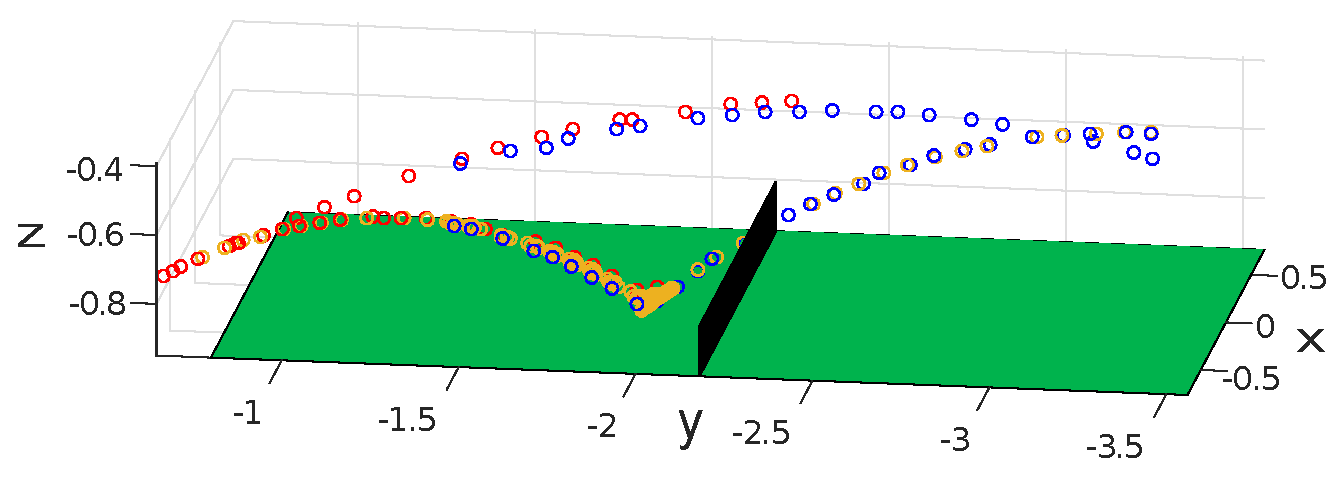
\includegraphics[scale=0.35]{trainBounce.eps}			
	\caption{Using Extended Kalman Smoothing (EKS) to estimate the parameters of the rebound model from actual noisy ball data during a demonstration recording. Ball observations are acquired from two different sets of cameras on opposite sides of the table, shown as red and blue circles respectively. They are then smoothened with the EKS, shown in yellow, to obtain velocity estimates before rebound and just after rebound. Nonlinear least squares is then used to estimate the rebound model parameters $\coeffFrictionTable$ and $\coeffRestitutionTable$.} 
	\label{trainBounce}
\end{figure}

%\begin{figure}
%	\centering
%	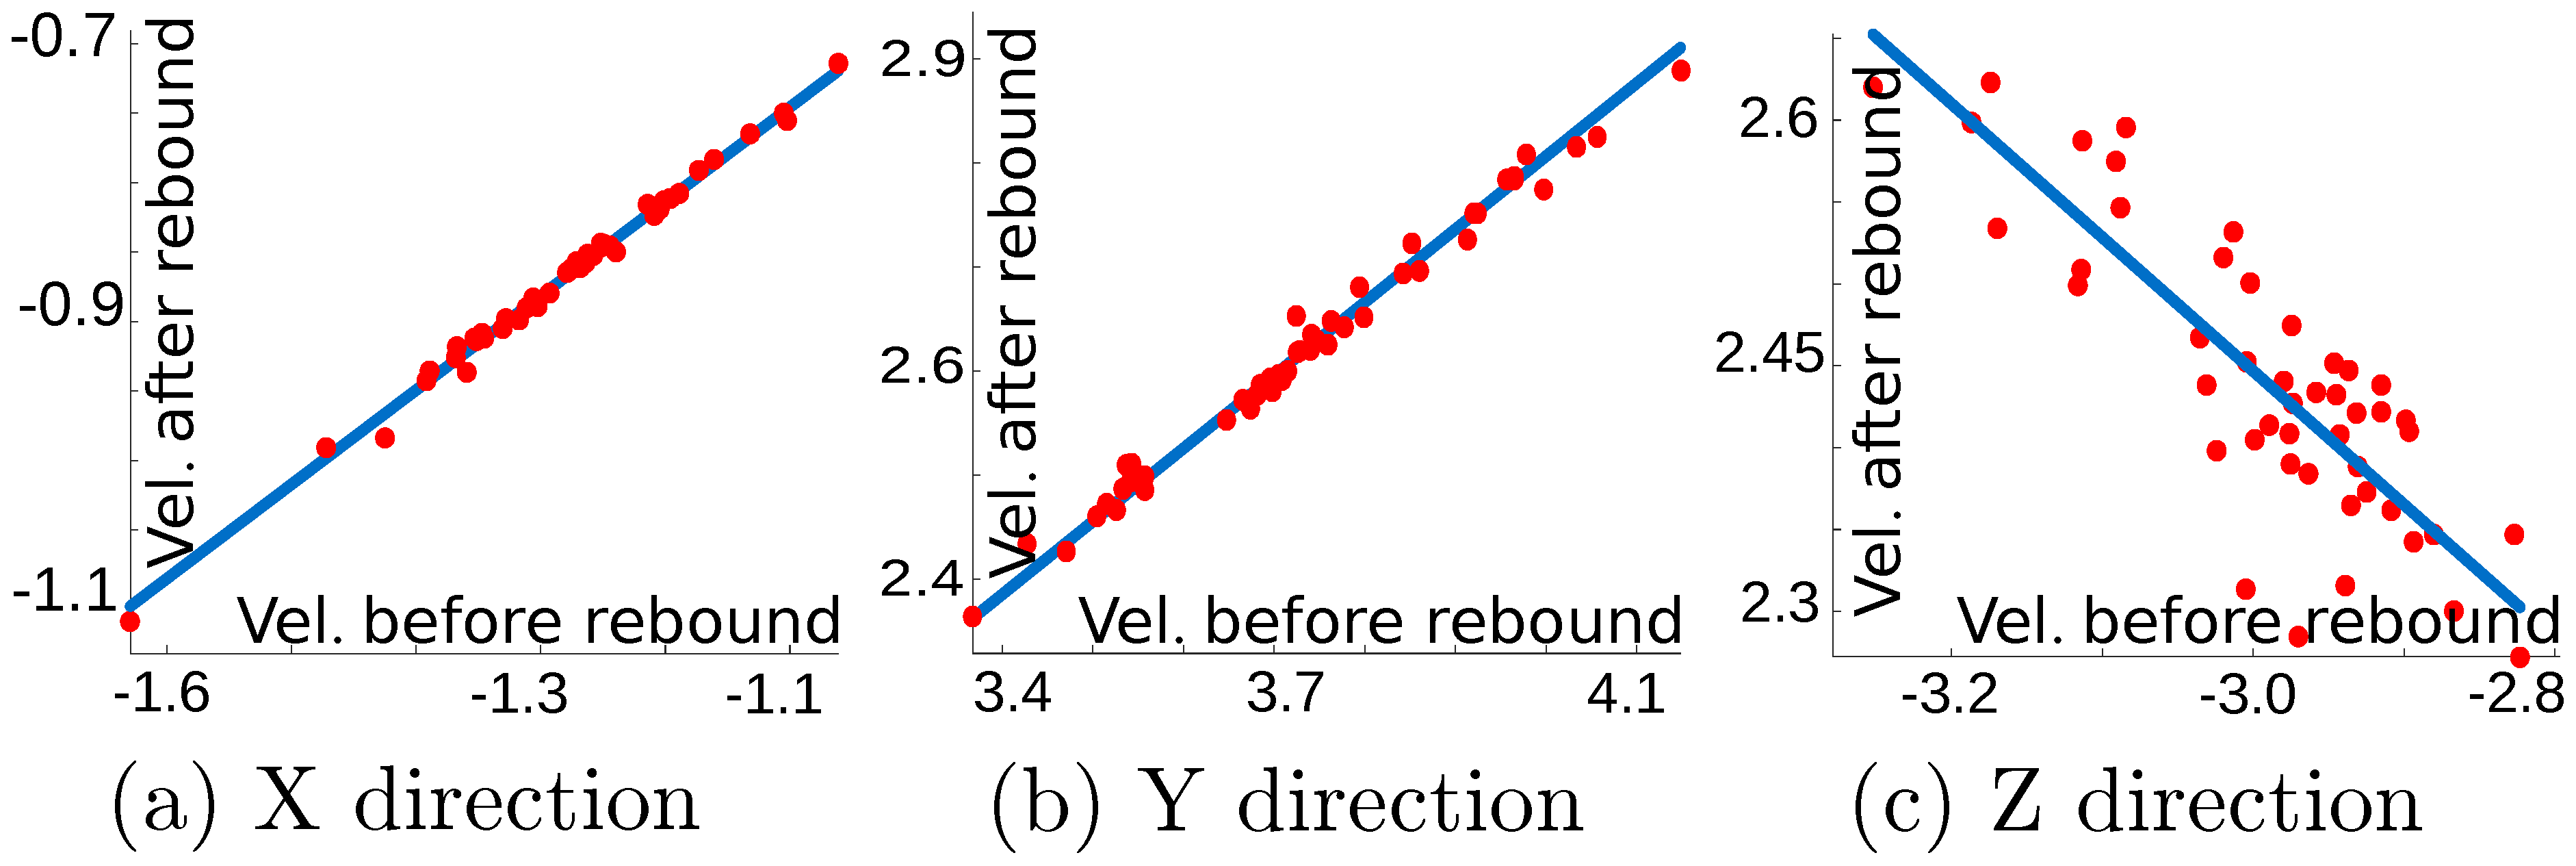
\includegraphics[scale=0.125]{velRebound2.eps}
%	\caption{The plots show the relationship between the velocities before and after rebound. The rebound model parameters are estimated from data with linear regression. It can be seen, especially in the X and Y directions, that the linear model is quite faithful to data. The estimated coefficients are $\epsilon_x = 0.82$, $\epsilon_y = 0.70$ and $\epsilon_z = 0.68$. When the topspin setting is increased in the ballgun to $3000$ rpm, the estimated coefficients increase to $\epsilon_x = 0.96$, $\epsilon_y = 1.18$ and $\epsilon_z = 1.20$.} %The topspin caused by our ball-launcher could be a complicating factor in the vertical direction Z. 
%	\label{fig:rebound}
%\end{figure}
%
In order to estimate the parameters, i.e., $\kappa$ and $\coeffRestitutionRacket$, of the ball-racket interaction model~\eqref{contactModel} we first use the dataset to estimate the striking times $\hitTime_i$. By considering the minimum distance between the ball samples and the demonstrated Cartesian robot trajectories
%
\begin{align}
j_h(i) &= \arg\min_{j} \|\ball_{ij} - \kin_p(\joint_{ij})\|_2, \\
\hitTime_i &\approx t_{ij_h(i)},
\label{strikingTimeEst}
\end{align}
%
\noindent for each trial $i = 1, \ldots N$ we can roughly estimate the striking times $\hitTime_i$. As in estimating the rebound model parameters, the Extended Kalman Smoother is then used to smoothen the ball demonstrations before and after the striking time separately. This procedure results in estimating the incoming and outgoing ball velocities, $\dot{\mathbf{b}}_{\mathrm{in}}(T_i), \, \dot{\ball}_{\mathrm{out}}(T_i)$ as well as the required racket quantities $\racketVel(T_i), \, \normal(T_i)$ at striking times $T_i$. Linear Least Squares is then used with regularizer $\lambda = 0.001$ to estimate the coefficients $\kappa$ and $\coeffRestitutionRacket$. See Table~\ref{tableEstimates} for the estimated values of all the ball model parameters.

An alternative approach would be to estimate all the model parameters together with a smoothing Expectation-Maximization (EM)~\citep{Shumway82} algorithm, yielding additionally covariance estimates for noisy ball observations. 
%
\begin{table}[b!]
	\small\sf %\centering
	%\renewcommand{\arraystretch}{1.3}
	\caption{Ball model parameter estimates}
	\label{tableEstimates}
	\begin{tabular}{c|l|l}
		\toprule
		\bfseries Parameter & \bfseries Description & \bfseries Estimate \\ %	{\small \bfseries Notation}
		\midrule
		$\drag$ & Air drag coefficient & 0.141 \\
		$\lift$ & Lift coefficient & 0.001 \\
		$\gravity$ & Gravity & -9.802 \\
		$\coeffFrictionTable$ & Coeff. of friction of table & 0.102 \\
		$\coeffRestitutionTable$ & Coef. of restitution of table & 0.883 \\
		$\kappa$ & Coeff. of friction of racket & 0.020 \\
		$\coeffRestitutionRacket$ & Coeff. of restitution of racket & 0.788 
		%\bottomrule
	\end{tabular}
\end{table}
\subsection{Real Robot Table Tennis}

In this section we describe and discuss our experiments on the robotic table tennis setup, see Figure~\ref{robot}. 
%We have used a graphical simulation environment to evaluate our algorithm in Table~\ref{tableSimResults}. The realistic simulation platform is designed to imitate the features of our robotic table tennis setup, see Figure~\ref{robot}. 

\paragraph{\textbf{Description of the Setup}.} Our robot is a seven degree of freedom Barrett WAM arm that can easily reach $10g$ m/$\textrm{s}^2$ accelerations. It is torque-controlled and cable-driven. A standard size racket ($7.6$ cm radius) is attached to the end-effector. The vision system tracks the balls at a rate of $60$ Hz and consists of four cameras on the corners on the ceiling. See~\citet{Lampert12} for platform details. The table and the tennis balls are standard sized, the balls have a radius of $2$ cm, the table geometry is approximately $276 \times 152 \times 76$ cm.

%Even though the cameras are capable of $200$ Hz monitoring, expensive debayering and filtering operations reduce the tracking to around $60$ Hz range.

In the robot experiments, we use a ball-launcher (see Figure~\ref{robot}) to throw balls to the the robot, approximately once every $2-3$ seconds. The balls generally come with a high variance, especially the velocities are quite unpredictable even without oscillating the ball-launcher. The robot base is at a distance of $115$ cm to the end of the table and $95$ cm above the table. Robot base is centered with respect to the table in the $x$ direction, see Figure~\ref{robot}. %The robot's forehand posture $\joint_0$ is chosen the same as in our simulations. 
%
\begin{figure}
	\begin{subfigure}[t]{0.5\textwidth}
		\centering
		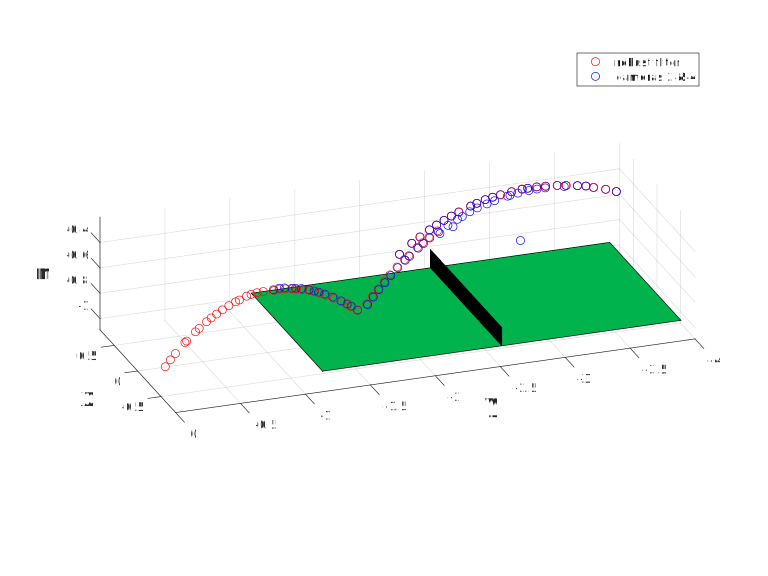
\includegraphics[scale=0.4]{robust_filtering_cam3.pdf}
		\caption{Filtering the noisy and corrupted data acquired from cameras 3 and 4 opposite to the robot side.}
		\label{outliersDataCam3}
	\end{subfigure}
	~ % remove this when using two column format
	\begin{subfigure}[t]{0.5\textwidth}
		\centering
		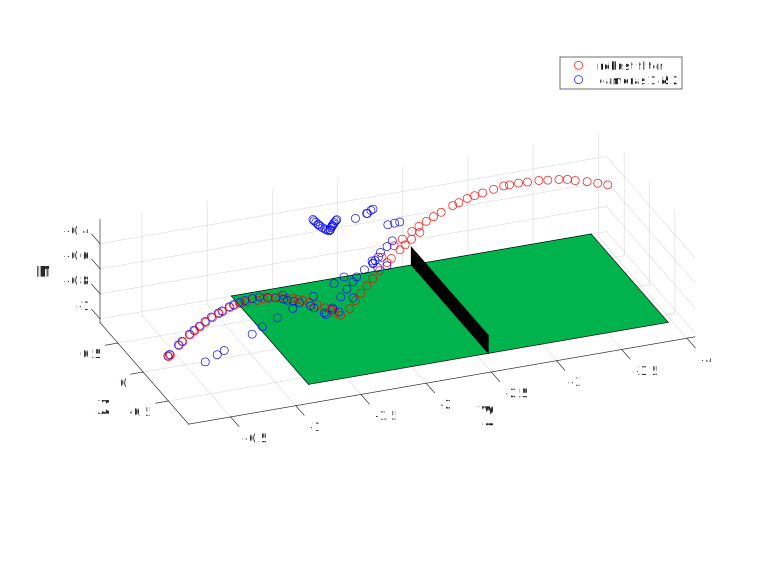
\includegraphics[scale=0.4]{robust_filtering_cam1.pdf}
		\caption{Filtering the noisy and corrupted data acquired from cameras 1 and 2 on the robot side.}
		\label{outliersDataCam1}
	\end{subfigure}
	\caption{Kalman Filtering with simultaneous outlier detection. The ball detection algorithm sometimes outputs outliers, typically more as the ball approaches the racket. Such corrupted data can be identified and discarded using the covariance of the Kalman Filter.}
	\label{outliersData}
\end{figure}
%
\paragraph{\textbf{Estimation and Outlier Detection}.} The ball detection algorithm detects the center of mass of the orange balls from each image separately and fuses them together to form two ball position estimates. These are then preprocessed and filtered with an Extended Kalman Filter (EKF) to estimate ball position and velocity. 

After the ball-launcher shoots a ball, $\numBallsMin \approx \minball$ ball observations are used to initialize the Kalman Filter state and launch the trajectory generation process, see Algorithms~\ref{alg1} and \ref{alg2}. Balls that suddenly appear on the opponent's court after disappearing for more than $\resetTime$ seconds from the cameras cause the Kalman Filter to reset. The filter state and the ball spin (assumed constant throughout motion) are then estimated together with a truncated Newton's method~\footnote{The optimization is launched on another thread using the \emph{TNEWTON} algorithm in NLopt~\citep{NLopt}.} using $\numBallsMin = \minball$ ball samples. We have experimentally confirmed the value of $\numBallsMin$ to be a good compromise between ball estimation accuracy (which requires waiting) and moving early (which can reduce the accelerations).
% TODO: plot here to show the trade-off curve

% RESETTING IS NOT MENTIONED IN THE ALGORITHMS - PUT A SUBBLOCK ?
The ball detection algorithm sometimes outputs outliers, possibly meters away from the actual ball. This typically happens more as the ball approaches the racket and new ball observations become more valuable. In order to prevent the outliers from ruining the estimation and the overall performance, we have implemented a robust EKF that does not perform measurement updates, if the ball observations lie more than $2$ standard deviations away from the predicted state. See Figure~\ref{outliersData} for actual table tennis ball data.
%
% PUT HERE AN EQUATION FOR OUTLIER DETECTION
%
We adjust the covariance estimates $\vec{\Sigma}(t)$ accordingly to make this procedure work in practice, e.g., covariances are initialized with a large $\vec{\Sigma}_{\mathrm{init}}$ value and the noise covariances $\vec{W}(t) \approx \diag(10^{-3})$ are adjusted to make sure that $\vec{\Sigma}(t)$ decreases suitably over time.
%
%Running the optimizers repeatedly allows us to correct for prediction and control errors, as in Model Predictive Control~\citep{Garcia89}.
%
%
\paragraph{\textbf{Online Correction of Computed Trajectories}.} Since the ball is moving at fast speeds, our online trajectory generation algorithms needs to be on the order of tens of milliseconds, in order to reliably intercept the incoming ball. The optimizers take on average $20-25$ ms to converge, and they can be re-run in the real-time platform whenever there are new reliable ball observations $\ball_\mathrm{obs}$. Before launching the trajectory optimizers, the path of the ball is predicted each time for $\predTime = 1.0$ seconds and the algorithms are initialized with current joint state estimates $\joint_{\textrm{cur}}, \dot{\joint}_{\textrm{cur}}$. During this correction process, we make sure that the updates are always incremental and feasible. For completeness, we list here our software checks. We make sure that:
%
\begin{enumerate}
	\item At least $N = \minball$ reliable ball observations are available. This typically happens before the balls pass the net.
	\item The new ball estimate is not too far off from the previous estimates.
	\item Our previous optimization thread has terminated before another one is launched.
	\item The resulting Cartesian trajectory intersects with the ball and all the task constraints are satisfied.
	\item The corrections are never excessive, i.e., the acceleration and joint limits \eqref{jointLimPointwise} and \eqref{jointLimTraj} are always respected.
	\item The ball estimate appears to be in front of the robot, i.e., $b_y < r_y$.
\end{enumerate}
%
If any of these conditions are violated, then the trajectories are not updated, and the previous striking trajectory is followed without interruption. 
%
%
The balls come with a high variance in position and especially in velocity. Typical incoming ball velocities imparted by the ball-launcher are around $4-6$ m/s range in the y-direction, which implies that in practice there can be a maximum of $10$ ball corrections till the ball passes the robot. The ball-launcher gives in addition a lot of $\emph{topspin}$ to the ball. This makes the corrections provided by the repeated optimization critical, as the ball models~\mbox{\eqref{flightModel} -- \eqref{contactModel}} are unable to capture some of the aerodynamic effects due to spin. Figure~\ref{predErrorReduction} shows the decrease in mean squared prediction error as more ball observations are acquired.
%
\begin{figure}
	\centering
	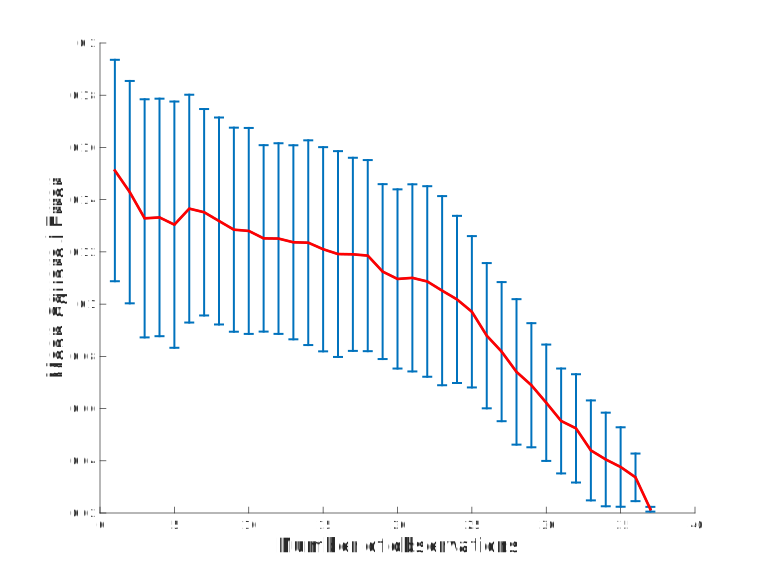
\includegraphics[scale=0.4]{predErrorReductionSpin.pdf}
	\caption{Mean squared prediction error (red curve) is reduced as more balls are observed. The ball observations are used until contact with racket occurs and the results are averaged over $100$ different real ball trials. Correcting for ball prediction error is critical for a robust table tennis performance, as the balls typically come with a high spin. Balls seems to lose some spin after rebound and the prediction error decreases faster. In this case this phenomenon can be observed after about $25$ ball observations, where the change in the average slope of the red curve can be seen.}
	\label{predErrorReduction}
\end{figure}
%
%topspin - roughly at $3000$ rates per minute
%
%Two example Cartesian trajectories computed by $\Alg$ are shown in Figure~\ref{fig:0} and Figure~\ref{fig:3}. The figures are snapshots of our simulation platform. Resulting trajectories naturally incorporate a swingback motion whenever needed, without explicit programming. More natural strikes can be computed in our framework. In the case shown in Figure~\ref{fig:0} for example, setting a VHP in front of the robot would result in very high accelerations, whereas the computed optimal trajectory intercepts with the ball trajectory behind the initial pose of the robot.
%
%\begin{figure}
%  \begin{subfigure}[t]{0.45\textwidth}
%    \centering
%    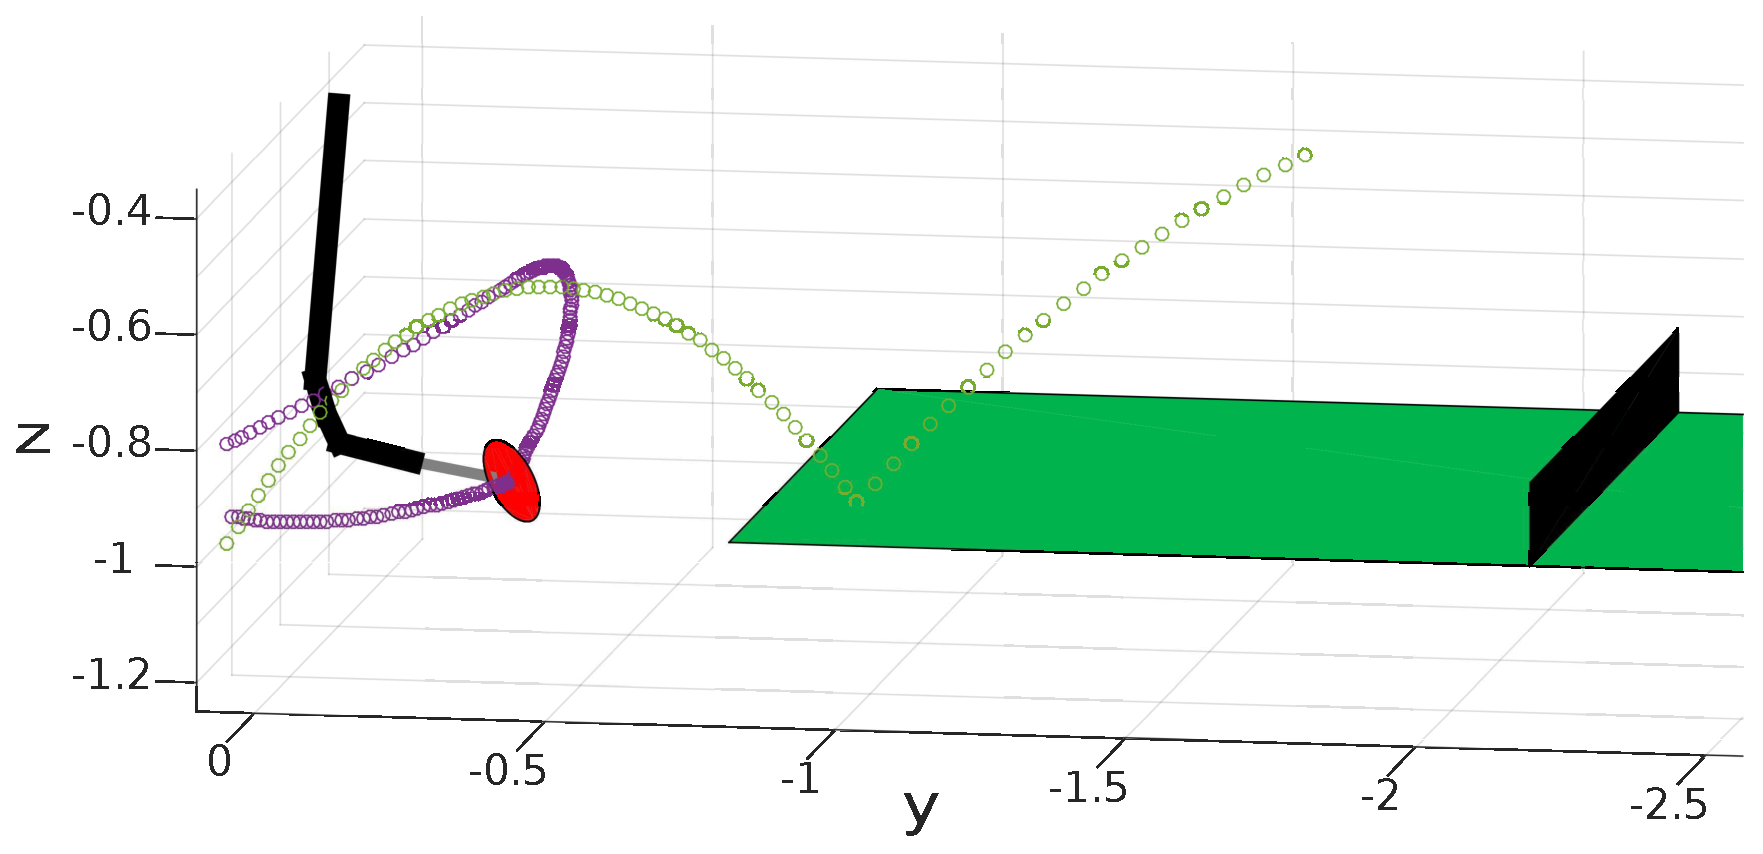
\includegraphics[width=\textwidth]{racket_ball_traj_0.eps}
%    \caption{Rest posture}
%    \label{fig:1}
%  \end{subfigure}
%  ~ % remove this when using two column format
%  \begin{subfigure}[t]{0.45\textwidth}
%  	\centering
%    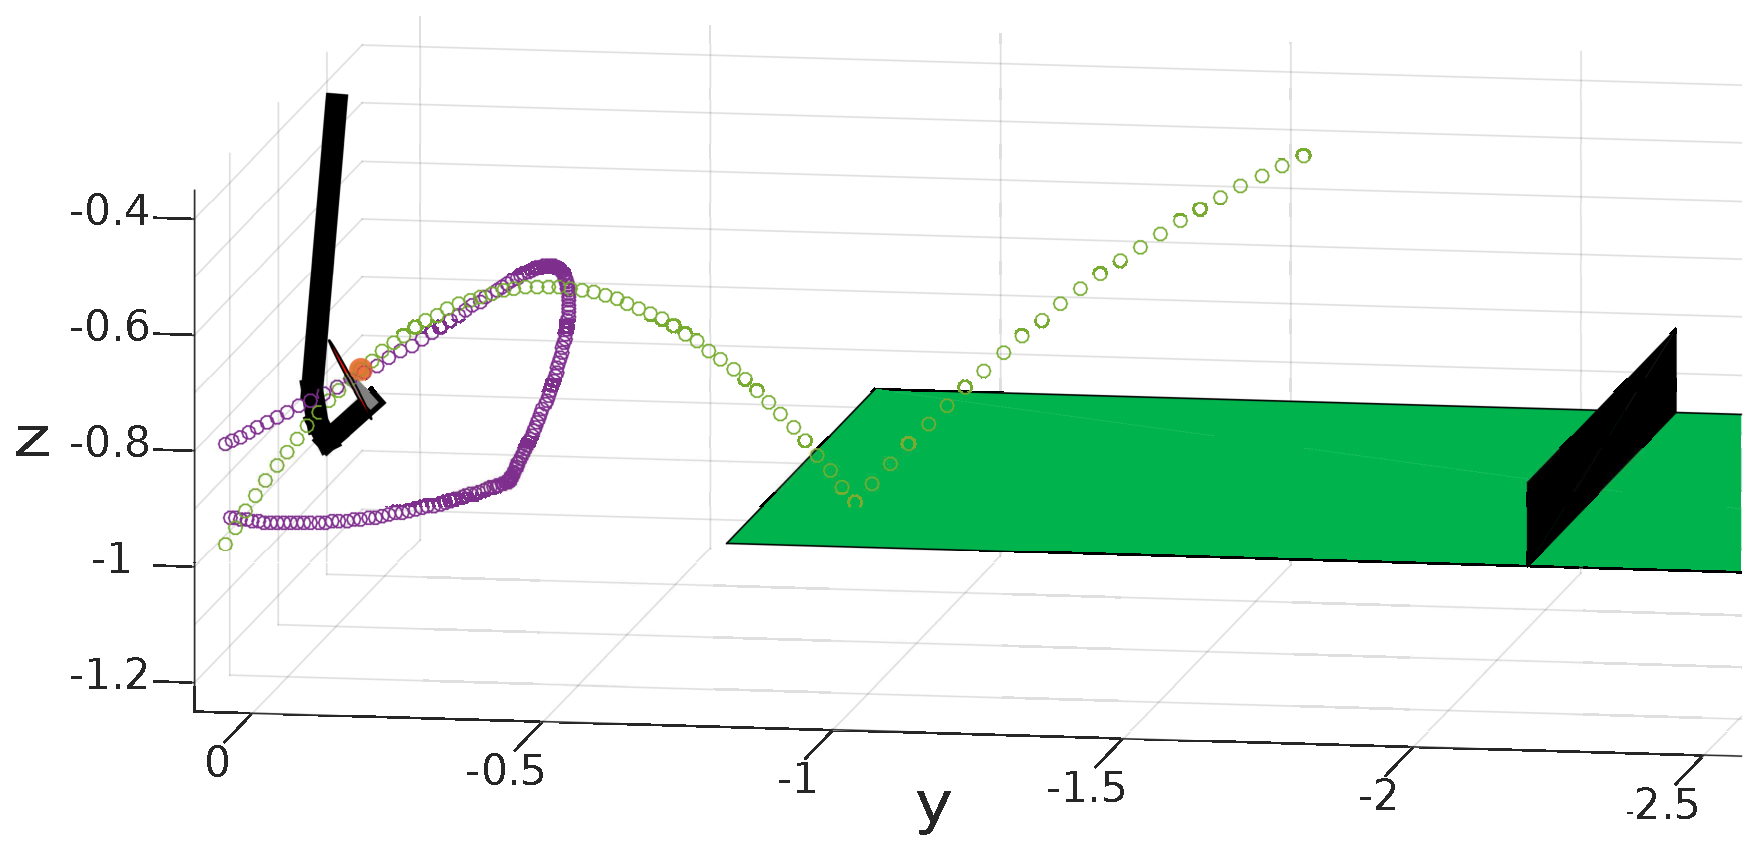
\includegraphics[width=\textwidth]{racket_ball_traj_1.eps}
%    \caption{Posture at striking time}
%    \label{fig:2}
%  \end{subfigure}
%  \caption{An example trajectory generated by the optimal control based framework is shown in purple. The resulting trajectory, minimizing the accelerations throughout, incorporates naturally a swingback pattern that may not be included in other methods fixing a virtual hitting plane (VHP).}
%  \label{fig:0}
%\end{figure}
%
%\begin{figure}[t!]
%\centering
%\includegraphics[scale=0.15]{racket_ball_traj_2.eps}	
%\caption{Another computed optimal trajectory. In this case, there is less swingback and the alignment with the ball trajectory is higher.}
%\label{fig:3}
%\end{figure}
%
\paragraph{\textbf{Discussion of Results}.} We compare and evaluate the performance of the two players $\alg$ and $\algTwo$ in the robot table tennis setup, see Figures~\ref{compare-players-real} and~\ref{exampleTT}. Results are averaged over $200$ trials where the ball-launcher is fixed at different positions or is oscillating, and the robot is placed at three different initial postures. For $\alg$, we also consider the variation in performance due to selecting different desired landing positions and landing times. Overall, $\alg$ is able to return about $40-60 \%$ of the balls to the opponent's court. Setting the desired landing position on the right side of the table, with a desired landing time of $T_{\textrm{land}} = 0.4$ seconds, leads to the best performance ($\sim 60\%$) in our table tennis setup. Increasing the time and setting the desired landing position closer to the centre of the opponents court makes the player less robust, decreasing the accuracy down to $40-50\%$ and increasing the variance of the landing locations, see Figure~\ref{distr_returns}. We believe this decrease in the performance is due to inaccuracies in the racket model.
%
% 
\begin{figure}
	\centering
	\setlength\figureheight{4cm}
	\setlength\figurewidth{5cm}
	% This file was created by matlab2tikz.
%
%The latest updates can be retrieved from
%  http://www.mathworks.com/matlabcentral/fileexchange/22022-matlab2tikz-matlab2tikz
%where you can also make suggestions and rate matlab2tikz.
%
\definecolor{mycolor1}{rgb}{0.20810,0.16630,0.52920}%
\definecolor{mycolor2}{rgb}{0.21783,0.72504,0.61926}%
\definecolor{mycolor3}{rgb}{0.97630,0.98310,0.05380}%
\definecolor{mycolor4}{rgb}{0.00000,0.44700,0.74100}%
%
\begin{tikzpicture}

\begin{axis}[%
width=0.951\figurewidth,
height=\figureheight,
at={(0\figurewidth,0\figureheight)},
scale only axis,
bar width=0.8,
xmin=0.5,
xmax=3.5,
xtick={1,2,3},
xticklabels={{FP},{DP},{VHP}},
ymin=0,
ymax=90,
axis background/.style={fill=white},
axis x line*=bottom,
axis y line*=left
]
\addplot[ybar stacked, fill=mycolor1, draw=black, area legend] table[row sep=crcr] {%
1	50\\
2	0\\
3	0\\
};
\addplot[forget plot, color=white!15!black] table[row sep=crcr] {%
0.5	0\\
3.5	0\\
};
\addplot[ybar stacked, fill=mycolor2, draw=black, area legend] table[row sep=crcr] {%
1	0\\
2	80\\
3	0\\
};
\addplot[forget plot, color=white!15!black] table[row sep=crcr] {%
0.5	0\\
3.5	0\\
};
\addplot[ybar stacked, fill=mycolor3, draw=black, area legend] table[row sep=crcr] {%
1	0\\
2	0\\
3	30\\
};
\addplot[forget plot, color=white!15!black] table[row sep=crcr] {%
0.5	0\\
3.5	0\\
};
\addplot [color=mycolor4, line width=1.0pt, draw=none, forget plot]
 plot [error bars/.cd, y dir = both, y explicit]
 table[row sep=crcr, y error plus index=2, y error minus index=3]{%
1	50	10	10\\
2	80	10	10\\
3	30	10	20\\
};
\end{axis}
\end{tikzpicture}%
	\caption{Summary of real robot table tennis experiment results comparing three table tennis players. Bar plot values show the successful return $\%$ averaged over different starting postures and initial ball positions. The error bars indicate the standard deviation over a total of $200$ trial runs.}
	\label{compare-players-real}
\end{figure}
%

The $\AlgTwo$ ($\algTwo$) is able to return about $80-90 \%$ of the balls, the performance varying depending on the incoming balls and the ballgun settings. The gain in accuracy is due to the increased flexibility of the algorithm, as well as the additional resting posture optimization which simplifies the task significantly. The algorithm finds counterintuitive resting postures that lead to smaller movements with less control error, see Figure~\ref{resting_posture_dp} for four consecutive trials of $\algTwo$. The duration of the returning trajectory is set to one second for all players: $\restTime = 1.0$ s. The weighting matrix $\vec{R}$ is set to identity and the weights for hitting and landing penalties are both set to ten: $\weightHit = 10, \weightLand = 10$.
%

VHP can return about $10-40\%$ of the balls. The best setting for the hitting plane location depends strongly on the ballgun settings, which affect the distribution of the incoming ball. In our experiments the hitting plane at $y = 30$ cm in front of the robot lead to the best performance ($\sim 40\%$). However, the accuracy can drop down significantly (to $10\%$ ) if the ballgun is oscillating, or the initial ball velocities are not appropriate for the particular VHP setting.
%
%
\begin{figure*}
	\centering
	\begin{minipage}[b]{.3\linewidth}
		\begin{subfigure}[t]{0.9\textwidth}
		\includegraphics[scale=0.15]{ball_lands_centre_des.pdf}
		\caption{$\alg$ with the desired ball landing location at the centre of the opponent's court.}
		\label{ball_land_des_centre}
		\end{subfigure}
	\end{minipage}%
	\begin{minipage}[b]{.3\linewidth}
		\begin{subfigure}[t]{0.9\textwidth}
		\includegraphics[scale=0.15]{ball_lands_right_des.pdf}
		\label{ball_land_des_right}
		\caption{$\alg$ with the desired ball landing location at the right side.}
		\end{subfigure}
	\end{minipage}
	\begin{minipage}[b]{.3\linewidth}
		\begin{subfigure}[t]{0.8\textwidth}
		\includegraphics[scale=0.15]{ball_lands_dp.pdf}
		\label{ball_land_dp}
		\caption{$\algTwo$ with a more flexible returning criterion.}
		\end{subfigure}
	\end{minipage}
	\caption{Overall, $\alg$ is able to return about $40-60 \%$ of the balls to the opponent's court. Setting the desired landing position on the right side of the table, with a desired landing time of $T_{\textrm{land}} = 0.4$ seconds, leads to the best performance ($\sim 60\%$) in our table tennis setup. Some example landing locations are indicated in orange in (b). Setting the desired landing position closer to the centre of the opponents court decreases the accuracy down to $40-50\%$, increasing also the variance of the landing locations, as shown in (a). $\algTwo$ in (c) with a landing accuracy of $80 \%$ has the highest variance in terms of the ball landing locations, as its returning criterion considers the whole opponent's court.}
	\label{distr_returns}
\end{figure*}
%
For all three algorithms, without applying any corrections, the robot is able to hit most balls but cannot return most balls successfully to the other side (only $5\%$ of the balls are returned). Applying the corrections about three times, and at least once after rebound, increases the performance to the indicated values, see Figure~\ref{compare-players-real}. This indicates that the rebound model chosen might not be accurate with high topspins that the ballgun imparts to the ball (around $3000$ rpm). 
%
%
\begin{figure*}
	\begin{minipage}[b]{.5\linewidth}
		\begin{subfigure}[t]{0.5\textwidth}
			\includegraphics[scale=0.28]{screenshots_new.pdf}
			\label{screenshots}
		\end{subfigure}
	\end{minipage}%
	\begin{minipage}[b]{.5\linewidth}
		%\begin{subfigure}[t]{0.5\textwidth}
		\includegraphics[scale=0.20]{act_vs_des_both.pdf}
		\label{act-vs-des-cartesian}
		%\caption{Reference and the actual striking trajectory in Cartesian space.}
		%\end{subfigure}
	\end{minipage}
	\caption{Two example table tennis trials recorded in the table tennis setup are shown on the left hand side. The top two screenshots show the $\Alg \ (\alg)$ in action, and the bottom four the $\AlgTwo \ (\algTwo)$. Unlike $\alg$, $\algTwo$ does not bring the robot back to the same initial posture (screenshots 3 vs. 6). Successful strike and the valid landing on the opponent's court for $\algTwo$ can be seen in the screenshots $4-6$. Balls are highlighted with green dashed circles for visibility. The plot in the upper right figure shows the recordings from the cameras and the robot sensors, corresponding to the hitting movement in screenshots 1 and 2. The blue dots are the ball observations coming from cameras 3 and 4. The desired Cartesian trajectory is drawn in red, and the actual trajectory, in black.}
	\label{exampleTT}
\end{figure*}
%
% two example trials from the video recording
Two example trials are shown in Figure~\ref{exampleTT}. The deviation from the desired hitting point, shown as an orange dot, was for the first example within three cm of the racket centre, resulting in a hit. The deviations in the reference velocities are higher and lead to approximately $10$ cm/s difference in Cartesian space. The successful strike and the landing on the opponent's court can be seen in the upper right figure. In the first example, player $\alg$ tries to return the ball to the right side of the opponents court, with a desired landing time of $T_{\textrm{land}} = 0.4$ seconds. The blue dots are the ball observations acquired from cameras 3 and 4, which are located on the corners of the ceiling on the robot side. In the second example (screenshots $3-6$), the player $\algTwo$ also returns the ball successfully, but unlike the other player, $\algTwo$ does not bring the robot back to the same initial posture.
%
%
\begin{figure}
	\centering
	\includegraphics[scale=0.12]{resting_postures.pdf}
	\caption{Four consecutive lands shown for the $\AlgTwo$ ($\algTwo$). In each trial, the arm goes back to a different resting posture.}
	\label{resting_posture_dp}
\end{figure}%
%
Control errors on the joint positions and velocities for this example are shown in Figure~\ref{control-error}. After the desired trajectories are calculated, high gain PD-control is applied along with an inverse dynamics controller (computed-torque). The inverse dynamics model is not very precise, but the feedback with high gains compensates for it well, especially in the shoulders and the elbow. %by running the optimization repeatedly, the robot can compensate and prevent the accumulation of control errors. 
%
%
%
%
\begin{figure}
  	\centering
  	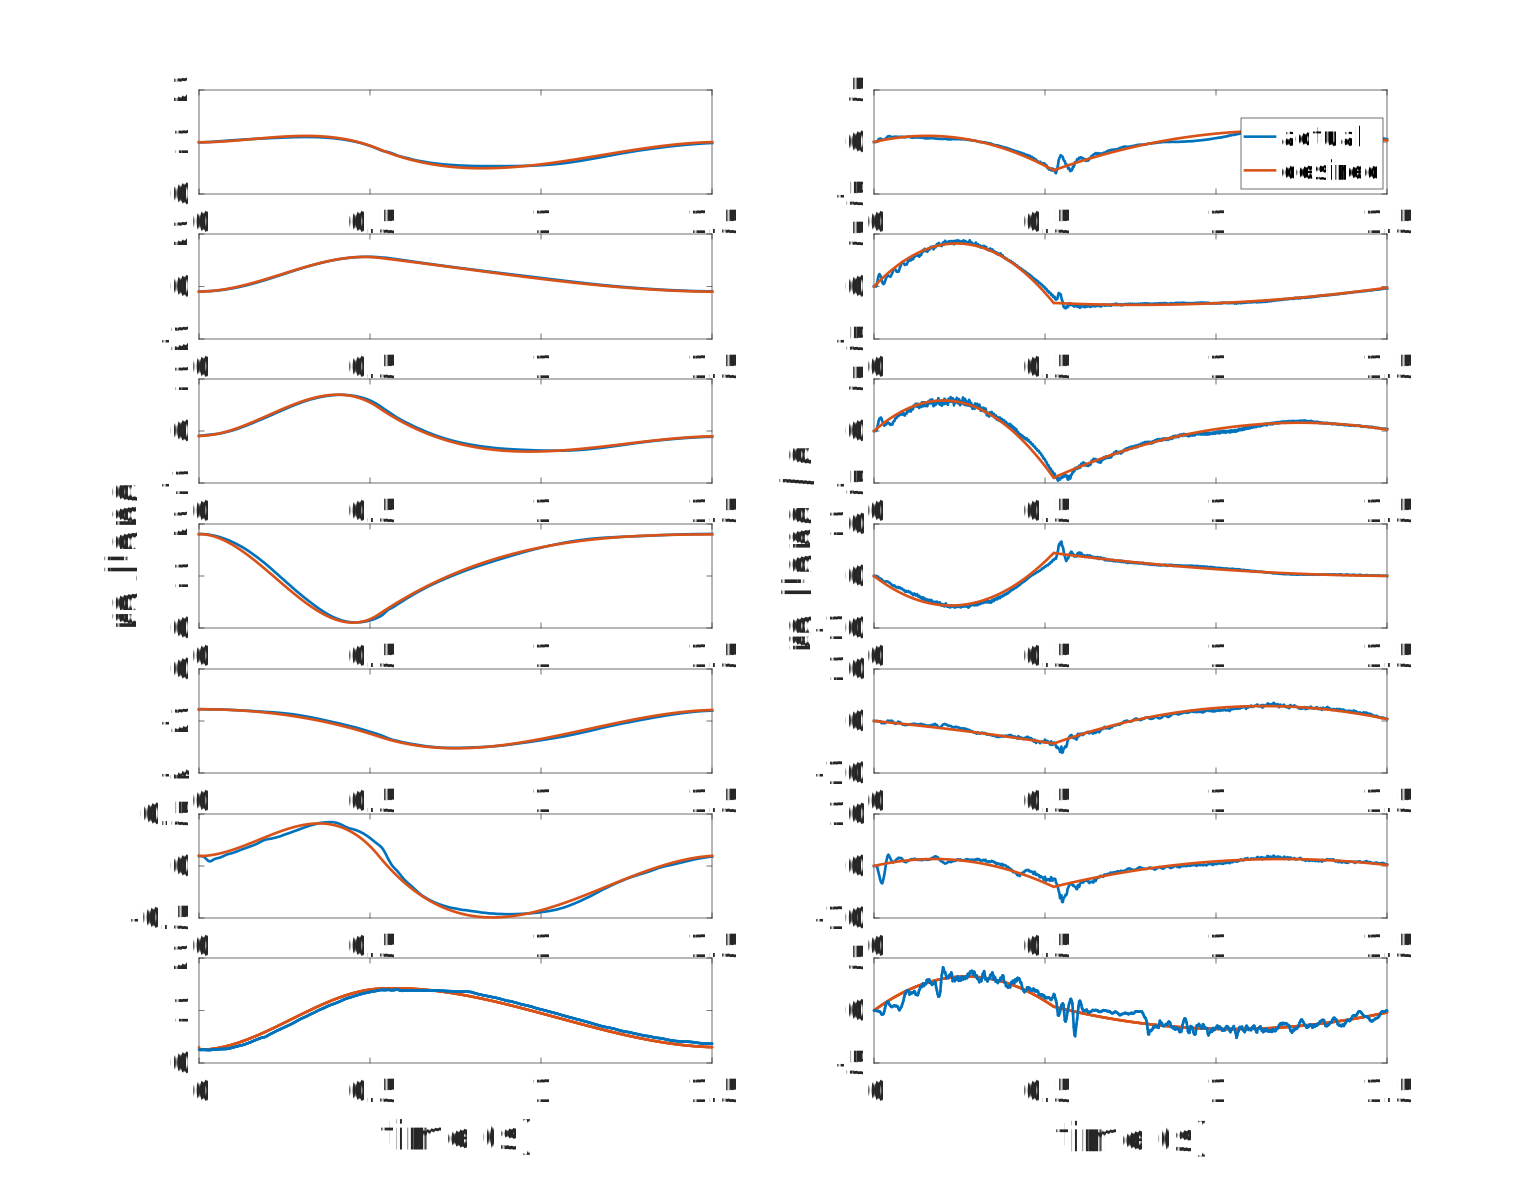
\includegraphics[scale=0.20]{act_vs_des_joints.pdf}
  	\caption{Tracking errors are shown for each joint. The desired joint positions and velocities are tracked with a PD controller. The deviation from the desired hitting point, shown as an orange dot in Figure~\ref{exampleTT}, was for this example within three centimeters of the racket centre, resulting in a hit.}
  	\label{control-error}
\end{figure}
%
% EXPERIMENTS - SHOWING IMPROVEMENT OVER PREVIOUS EXP
\section{Conclusion}\label{end}

In this paper we have presented two new algorithms ($\alg$ and $\algTwo$) for generating table tennis striking trajectories that extend previous work in table tennis strike movement generation. 

\subsection{Summary of the Contributions}

The two table tennis players use an optimal-control based approach for generating striking trajectories. The striking and return trajectories are third order polynomials that intercept the ball at the optimized hitting point at the optimized hitting time. Unlike previous approaches, our optimization based framework respects the joint limits, while leading to efficient movements with low accelerations. Furthermore, by varying the hitting time $T$ the problem of finding feasible joint trajectories is simplified. Further constraints can be easily imposed on the system, and we have considered, for instance, racket constraints for $\alg$ and an additional resting posture optimization for $\algTwo$. 

The optimizations can be run online in the robotic setup shown in Figure~\ref{robot} and given new joint position and ball position measurements, the trajectories are updated. Correcting for new ball positions, by repeating optimization, makes our table tennis players more robust to execution errors and inaccuracies in ball estimation $\&$ prediction. We show the performance of our two table tennis players in the real robot platform and compare with previous approaches.

\subsection{Outlook \& Future Work}

The two players $\Alg$ and $\AlgTwo$ can generate trajectories more flexibly than before and lead to two different play-styles which could potentially be utilized by a higher-level strategy. We believe that this is a promising direction, where a higher level learning algorithm could switch between different trajectory generation schemes. The weights and the additional parameterization for the two algorithms can be explored based on feedback on the robot's performance. Reinforcement learning~\citep{Sutton98} with rewards based on observed ball landing positions, provides a suitable framework to tune the proposed algorithms' performance online.

Finally, the cost functionals that we have introduced consider the accelerations as the quantity to be minimized. Whenever the cancellation in feedback linearization is imperfect due to inaccurate robot dynamics models, execution errors will prevent the robot from achieving the desired trajectories or the minimal accelerations. A more robust and adaptive way to include execution errors in trajectory generation will be considered in future work.

% CRITICAL DISCUSSION: 
% too much model dependent

\bibliographystyle{elsarticle-harv}
%\bibliographystyle{IEEEtran}
%\bibliographystyle{SageH}
\bibliography{./ttRef}

\parpic{\includegraphics[width=1in,clip,keepaspectratio]{okan_cut.pdf}}
\noindent {\bf Okan Ko\c c} received his B.S. degree in Electrical Engineering from Bogazici University, Turkey in 2009. He received his M.S. degree in 2013 in Applied Mathematics from ETH Z\"urich. He is currently a Ph.D. Candidate in Intelligent Autonomous Systems at Technische Universit\"at Darmstadt. His research interests are in the areas of optimal control and learning control.

\parpic{\includegraphics[width=1in,clip,keepaspectratio]{guilherme.jpg}}
\noindent {\bf Guilherme Maeda} is a research scientist at the Intelligent Autonomous Systems group (IAS) in TU Darmstadt since November 2013. His goal is to enable robots to learn challenging tasks by interacting with humans and with the environment. To this end, his research bridges the areas of control, learning, and human-robot collaboration. Guilherme received his PhD from the Australian Centre for Field Robotics (ACFR). He did his work under the supervision of Hugh Durrant-Whyte, Surya Singh, David Rye, and Ian Manchester. 

\parpic{\includegraphics[width=1in,clip,keepaspectratio]{jan.jpg}}
\noindent {\bf  Jan Peters} is a full professor (W3) for Intelligent Autonomous Systems at the Computer Science Department of the Technische Universit\"at Darmstadt and at the same time an adjunct senior research scientist at the Max-Planck Institute for Intelligent Systems, where he heads the interdepartmental Robot Learning Group between the departments of Empirical Inference and Autonomous Motion. Jan Peters has received a few awards, most notably, he has received the Dick Volz Best 2007 US PhD Thesis Runner Up Award, the 2012 Robotics: Science \& Systems - Early Career Spotlight, the 2013 IEEE Robotics \& Automation Society's Early Career Award, and the 2013 INNS Young Investigator Award. 

\end{document}
